% =====================================================================
%  PAPER III -- Certificates as Constraints:
%  Feasibility-Preserving Multi-Agent Reinforcement Learning for
%  UAV Swarms Whose Guarantees Degrade
%
%  Target venue : NeurIPS (main track).
%  Build        : latexmk -pdf main.tex      (pdfLaTeX + BibTeX)
%  Style        : if neurips_2027.sty (or neurips_2026.sty) is present in this
%                 folder it is used; otherwise an equivalent article layout is
%                 used so the file always compiles. Download the official style
%                 from the NeurIPS call for papers before submission.
%
%  Every number in the text is a macro from numbers.tex, generated by
%  paperIII/experiments/make_numbers.py from the committed result CSVs.
%  Every plotted point is read from figdata/*.dat. Do not edit numbers by
%  hand: re-run paperIII/experiments/run_all.sh (and run_marl.sh).
% =====================================================================
\documentclass[10pt]{article}
\IfFileExists{neurips_2027.sty}{\usepackage{neurips_2027}}{%
 \IfFileExists{neurips_2026.sty}{\usepackage{neurips_2026}}{%
  \usepackage[letterpaper,textwidth=5.5in,textheight=9in,top=1in]{geometry}%
  \usepackage{times}}}
\usepackage[utf8]{inputenc}
\usepackage[T1]{fontenc}
\usepackage[numbers,sort&compress]{natbib}
\usepackage{amsmath,amssymb,amsfonts,amsthm,mathtools}
\usepackage{bm}
\usepackage{graphicx}
\usepackage{booktabs}
\usepackage{tabularx}
\usepackage{array}
\usepackage{multirow}
\usepackage{xcolor}
\usepackage{tikz}
\usepackage{pgfplots}
\pgfplotsset{compat=1.17}
\usepgfplotslibrary{groupplots,fillbetween}
\usetikzlibrary{arrows.meta,positioning,fit,backgrounds,shapes.geometric,calc}
\usepackage{algorithm}
\usepackage{algpseudocode}
\usepackage{enumitem}
\usepackage{microtype}
\usepackage{placeins}
\usepackage[hidelinks]{hyperref}
\usepackage[capitalise,noabbrev]{cleveref}

% generated by paperIII/experiments/make_numbers.py -- do not edit
\newcommand{\nAlphaMax}{20}
\newcommand{\nAlphaMin}{2}
\newcommand{\nBlindCov}{0.451}
\newcommand{\nBlindProjCov}{0.492}
\newcommand{\nBlindProjRatio}{1.00}
\newcommand{\nBlindProjSwitch}{5.0}
\newcommand{\nBlindProjViol}{0.00}
\newcommand{\nBlindProjViolMean}{0.00}
\newcommand{\nBlindRatio}{0.51}
\newcommand{\nBlindSwitch}{0.0}
\newcommand{\nBlindTrainRate}{16.47}
\newcommand{\nBlindTrainViol}{4{,}744{,}505}
\newcommand{\nBlindViol}{13.75}
\newcommand{\nBlindViolMean}{12.67}
\newcommand{\nCbbaCov}{0.539}
\newcommand{\nCbbaCovHi}{0.561}
\newcommand{\nCbbaCovLo}{0.525}
\newcommand{\nCbbaEvalViol}{0}
\newcommand{\nCbbaEvalViolPct}{0.000}
\newcommand{\nCbbaRatio}{1.00}
\newcommand{\nCbbaSeeds}{1}
\newcommand{\nCnsAgreedMaxExcess}{0}
\newcommand{\nCnsDropDev}{4}
\newcommand{\nCnsDropExcess}{2}
\newcommand{\nCnsDropF}{2}
\newcommand{\nCnsDropLost}{24}
\newcommand{\nCnsDropMesh}{2}
\newcommand{\nCnsEqFourFOne}{96}
\newcommand{\nCnsEqFourFTwo}{51}
\newcommand{\nCnsEqFullFOne}{100}
\newcommand{\nCnsEqFullFTwo}{100}
\newcommand{\nCnsEqRingFOne}{66}
\newcommand{\nCnsEqRingFTwo}{26}
\newcommand{\nCnsEqSixFOne}{100}
\newcommand{\nCnsEqSixFTwo}{74}
\newcommand{\nCnsFullRoundsMax}{6}
\newcommand{\nCnsFwdMaxExcess}{0}
\newcommand{\nCnsHonestViol}{0}
\newcommand{\nCnsInst}{200}
\newcommand{\nCnsLiarViol}{4{,}819}
\newcommand{\nCnsRobFour}{2}
\newcommand{\nCnsRobFull}{6}
\newcommand{\nCnsRobRing}{1}
\newcommand{\nCnsRobSix}{3}
\newcommand{\nCnsRobustAgree}{1.00}
\newcommand{\nCollB}{4}
\newcommand{\nCollGeneric}{3.89}
\newcommand{\nCollNom}{7.89}
\newcommand{\nCollRand}{6.37}
\newcommand{\nCollWorst}{5.55}
\newcommand{\nCovPdt}{0.263}
\newcommand{\nCovPdtFive}{0.371}
\newcommand{\nCovPone}{0.168}
\newcommand{\nCovPtwo}{0.083}
\newcommand{\nCovRel}{0.209}
\newcommand{\nCovStd}{0.393}
\newcommand{\nCovStdFive}{0.390}
\newcommand{\nDtMax}{0.200}
\newcommand{\nExpCut}{8.1}
\newcommand{\nExpCutFive}{6.4}
\newcommand{\nExpNoJPdt}{0}
\newcommand{\nExpNoJPdtFive}{0}
\newcommand{\nExpNoJPone}{0}
\newcommand{\nExpNoJPtwo}{0}
\newcommand{\nExpNoJRel}{2182}
\newcommand{\nExpNoJStd}{2930}
\newcommand{\nExpNoJStdFive}{2842}
\newcommand{\nExpPdt}{0.19}
\newcommand{\nExpPdtFive}{0.09}
\newcommand{\nExpPone}{0.14}
\newcommand{\nExpPtwo}{0.10}
\newcommand{\nExpRel}{1.18}
\newcommand{\nExpStd}{1.51}
\newcommand{\nExpStdFive}{0.56}
\newcommand{\nExpl}{3.26}
\newcommand{\nFixedCov}{0.163}
\newcommand{\nFixedRatio}{0.31}
\newcommand{\nFixedSwitch}{0.0}
\newcommand{\nFixedViol}{8.03}
\newcommand{\nFixedViolMean}{8.03}
\newcommand{\nGammaSup}{1.625}
\newcommand{\nGnpCov}{0.169}
\newcommand{\nGnpRatio}{0.98}
\newcommand{\nGnpSwitch}{8.6}
\newcommand{\nGnpViol}{0.00}
\newcommand{\nGnpViolMean}{0.00}
\newcommand{\nGradRandSix}{5.36}
\newcommand{\nGradTight}{100}
\newcommand{\nGradViol}{0}
\newcommand{\nGradWorstSix}{4.38}
\newcommand{\nHeurCov}{0.435}
\newcommand{\nHeurNoneCov}{0.459}
\newcommand{\nHeurNoneRatio}{0.51}
\newcommand{\nHeurNoneSwitch}{0.0}
\newcommand{\nHeurNoneViol}{13.97}
\newcommand{\nHeurNoneViolMean}{13.97}
\newcommand{\nHeurRatio}{1.00}
\newcommand{\nHeurSwitch}{2.3}
\newcommand{\nHeurViol}{0.00}
\newcommand{\nHeurViolMean}{0.00}
\newcommand{\nHiddenMax}{4.84}
\newcommand{\nHiddenMed}{3.94}
\newcommand{\nHystCovHalf}{0.379}
\newcommand{\nHystCovZero}{0.393}
\newcommand{\nHystHolds}{100}
\newcommand{\nHystSwHalf}{2.01}
\newcommand{\nHystSwZero}{2.38}
\newcommand{\nJumpMed}{41.8}
\newcommand{\nJumpOneMed}{20.9}
\newcommand{\nKappa}{5.30}
\newcommand{\nLagCov}{0.036}
\newcommand{\nLagProjCov}{0.393}
\newcommand{\nLagProjRatio}{0.99}
\newcommand{\nLagProjSwitch}{3.9}
\newcommand{\nLagProjViol}{0.00}
\newcommand{\nLagProjViolMean}{0.00}
\newcommand{\nLagRatio}{0.04}
\newcommand{\nLagSwitch}{0.0}
\newcommand{\nLagTrainRate}{13.55}
\newcommand{\nLagTrainViol}{3{,}903{,}179}
\newcommand{\nLagViol}{0.02}
\newcommand{\nLagViolMean}{0.73}
\newcommand{\nLatCFHundredK}{6.2}
\newcommand{\nLatCFThousand}{0.038}
\newcommand{\nLatCPU}{x86-64}
\newcommand{\nLatGNPHundredK}{40}
\newcommand{\nLatGNPTenK}{2.8}
\newcommand{\nLatGNPThousand}{0.21}
\newcommand{\nLatHKTenK}{1682}
\newcommand{\nLatHunThousand}{11.0}
\newcommand{\nLatHunTwelve}{0.038}
\newcommand{\nLatHunTwoK}{53}
\newcommand{\nLiarHonest}{0}
\newcommand{\nLiarInst}{4{,}000}
\newcommand{\nLiarMaxDev}{0}
\newcommand{\nLiftFleets}{64}
\newcommand{\nLiftIndFourHi}{0.1}
\newcommand{\nLiftIndFourLo}{0.0}
\newcommand{\nLiftIndFourPred}{0.0}
\newcommand{\nLiftIndFourSim}{0.1}
\newcommand{\nLiftIndFullPred}{0.934}
\newcommand{\nLiftIndFullSim}{0.927}
\newcommand{\nLiftIndQnone}{20}
\newcommand{\nLiftIndThreePred}{0.3}
\newcommand{\nLiftIndThreeSim}{0.4}
\newcommand{\nLiftOver}{3.4}
\newcommand{\nLiftSpFourHi}{57.5}
\newcommand{\nLiftSpFourLo}{37.8}
\newcommand{\nLiftSpFourPred}{38.6}
\newcommand{\nLiftSpFourSim}{47.5}
\newcommand{\nLiftSpFullHi}{0.334}
\newcommand{\nLiftSpFullLo}{0.175}
\newcommand{\nLiftSpFullPred}{0.074}
\newcommand{\nLiftSpFullSim}{0.250}
\newcommand{\nLiftSpQnone}{58}
\newcommand{\nLiftSpSixHi}{32.9}
\newcommand{\nLiftSpSixLo}{15.5}
\newcommand{\nLiftSpSixPred}{6.5}
\newcommand{\nLiftSpSixSim}{24.1}
\newcommand{\nLiftSpThreePred}{61.4}
\newcommand{\nLiftSpThreeSim}{55.3}
\newcommand{\nLiftUnder}{3.7}
\newcommand{\nLloc}{1.181}
\newcommand{\nMLagCov}{0.451}
\newcommand{\nMLagCovHi}{0.458}
\newcommand{\nMLagCovLo}{0.440}
\newcommand{\nMLagEvalViol}{6}
\newcommand{\nMLagEvalViolPct}{0.003}
\newcommand{\nMLagProjCov}{0.465}
\newcommand{\nMLagProjRatio}{0.99}
\newcommand{\nMLagRatio}{0.58}
\newcommand{\nMLagSeeds}{1}
\newcommand{\nMLagTrainRate}{4.80}
\newcommand{\nMLagTrainViol}{276{,}565}
\newcommand{\nMLagZeroCov}{0.450}
\newcommand{\nMLagZeroCovHi}{0.481}
\newcommand{\nMLagZeroCovLo}{0.422}
\newcommand{\nMLagZeroEvalViol}{3}
\newcommand{\nMLagZeroEvalViolPct}{0.002}
\newcommand{\nMLagZeroProjCov}{0.413}
\newcommand{\nMLagZeroProjRatio}{1.00}
\newcommand{\nMLagZeroRatio}{0.58}
\newcommand{\nMLagZeroSeeds}{1}
\newcommand{\nMLagZeroTrainRate}{5.86}
\newcommand{\nMLagZeroTrainViol}{337{,}727}
\newcommand{\nMaskCov}{0.464}
\newcommand{\nMaskProjCov}{0.499}
\newcommand{\nMaskProjRatio}{1.00}
\newcommand{\nMaskProjSwitch}{4.9}
\newcommand{\nMaskProjViol}{0.00}
\newcommand{\nMaskProjViolMean}{0.00}
\newcommand{\nMaskRatio}{0.62}
\newcommand{\nMaskSwitch}{0.7}
\newcommand{\nMaskTrainRate}{0.00}
\newcommand{\nMaskTrainViol}{0}
\newcommand{\nMaskViol}{0.00}
\newcommand{\nMaskViolMean}{0.00}
\newcommand{\nNBenign}{10{,}621}
\newcommand{\nNHidden}{1{,}346}
\newcommand{\nNHops}{15{,}392}
\newcommand{\nNSeeds}{5}
\newcommand{\nNoDevCov}{0.499}
\newcommand{\nNoDevRatio}{1.00}
\newcommand{\nNoDevSwitch}{4.9}
\newcommand{\nNoDevTrainRate}{0.00}
\newcommand{\nNoDevTrainViol}{0}
\newcommand{\nNoDevViol}{0.00}
\newcommand{\nNoDevViolMean}{0.00}
\newcommand{\nOursCov}{0.496}
\newcommand{\nOursCovHi}{0.525}
\newcommand{\nOursCovLo}{0.473}
\newcommand{\nOursRatio}{1.00}
\newcommand{\nOursTrainCP}{1.0\times10^{-7}}
\newcommand{\nOursTrainSteps}{2.9\times10^{7}}
\newcommand{\nPidLagCov}{0.000}
\newcommand{\nPidLagCovHi}{0.000}
\newcommand{\nPidLagCovLo}{0.000}
\newcommand{\nPidLagEvalViol}{0}
\newcommand{\nPidLagEvalViolPct}{0.000}
\newcommand{\nPidLagProjCov}{0.344}
\newcommand{\nPidLagProjRatio}{0.98}
\newcommand{\nPidLagRatio}{0.00}
\newcommand{\nPidLagSeeds}{2}
\newcommand{\nPidLagTrainRate}{14.33}
\newcommand{\nPidLagTrainViol}{1{,}650{,}843}
\newcommand{\nQmixCov}{0.420}
\newcommand{\nQmixCovHi}{0.439}
\newcommand{\nQmixCovLo}{0.406}
\newcommand{\nQmixEvalViol}{33{,}712}
\newcommand{\nQmixEvalViolPct}{9.755}
\newcommand{\nQmixMaskCov}{0.446}
\newcommand{\nQmixMaskCovHi}{0.462}
\newcommand{\nQmixMaskCovLo}{0.433}
\newcommand{\nQmixMaskEvalViol}{0}
\newcommand{\nQmixMaskEvalViolPct}{0.000}
\newcommand{\nQmixMaskProjCov}{0.510}
\newcommand{\nQmixMaskProjRatio}{1.00}
\newcommand{\nQmixMaskRatio}{0.57}
\newcommand{\nQmixMaskSeeds}{1}
\newcommand{\nQmixMaskTrainRate}{0.00}
\newcommand{\nQmixMaskTrainViol}{0}
\newcommand{\nQmixProjCov}{0.469}
\newcommand{\nQmixProjRatio}{1.00}
\newcommand{\nQmixRatio}{0.60}
\newcommand{\nQmixSeeds}{2}
\newcommand{\nQmixTrainRate}{12.56}
\newcommand{\nQmixTrainViol}{1{,}446{,}595}
\newcommand{\nRateMin}{5.01}
\newcommand{\nRatioPdt}{0.834}
\newcommand{\nRatioPdtFive}{0.983}
\newcommand{\nRatioPone}{0.654}
\newcommand{\nRatioPtwo}{0.377}
\newcommand{\nRatioRel}{0.983}
\newcommand{\nRatioStd}{0.983}
\newcommand{\nRatioStdFive}{0.977}
\newcommand{\nRhoFloor}{0.94}
\newcommand{\nSizeInd}{15}
\newcommand{\nSizeSp}{>30}
\newcommand{\nSwPdt}{1.61}
\newcommand{\nSwPdtFive}{0.94}
\newcommand{\nSwPone}{0.90}
\newcommand{\nSwPtwo}{0.39}
\newcommand{\nSwRel}{20.56}
\newcommand{\nSwStd}{2.38}
\newcommand{\nSwStdFive}{0.88}
\newcommand{\nThetaBen}{0.178}
\newcommand{\nVecBruteEight}{4.9}
\newcommand{\nVecBruteTwenty}{106}
\newcommand{\nVecClosed}{0.04}
\newcommand{\nVecGapTwelve}{0.77}
\newcommand{\nVecGapTwenty}{2.29}
\newcommand{\nVecInst}{400}
\newcommand{\nVecLossFracTwelve}{49}
\newcommand{\nVecLostTwelve}{0.65}
\newcommand{\nVecLostTwenty}{1.73}
\newcommand{\nVecLostTwentyMax}{5}
\newcommand{\nVecNestedTwelve}{74}
\newcommand{\nVecNestedTwenty}{10}
\newcommand{\nVecSigZeroLost}{0.0}
\newcommand{\nVerChecks}{9}
\newcommand{\nVerDisagree}{0}
\newcommand{\nVerInst}{10{,}000}
\newcommand{\nVerTotal}{83{,}872}


% ---------------- notation -------------------------------------------
\newcommand{\N}{\mathcal{N}}
\newcommand{\T}{\mathcal{T}}
\newcommand{\R}{\mathbb{R}}
\newcommand{\E}{\mathbb{E}}
\newcommand{\Prob}{\mathbb{P}}
\newcommand{\rhoi}{\rho_i}
\newcommand{\Lrho}{L_\rho}
\newcommand{\Proj}{\Pi}
\newcommand{\idle}{\varnothing}
\newcommand{\Qop}{\mathbf{Q}_{\mathrm{op}}}
\newcommand{\Qpop}{\mathbf{Q}_{\mathrm{pop}}}
\newcommand{\rcert}{r_{\mathrm{cert}}}
\newcommand{\TVp}{\mathrm{TV}^{+}}
\newcommand{\ie}{i.e.,\xspace}
\providecommand{\xspace}{}
\DeclareMathOperator*{\argmax}{arg\,max}

\newtheorem{theorem}{Theorem}
\newtheorem{lemma}{Lemma}
\newtheorem{proposition}{Proposition}
\newtheorem{corollary}{Corollary}
\theoremstyle{definition}
\newtheorem{definition}{Definition}
\newtheorem{assumption}{Assumption}
\theoremstyle{remark}
\newtheorem{remark}{Remark}

\title{Certificates as Constraints: Feasibility-Preserving Multi-Agent\\
Reinforcement Learning for UAV Swarms Whose Guarantees Degrade}

\author{Anonymous Author(s)\\ Submitted for double-blind review}
\date{}

\begin{document}
\maketitle

% =====================================================================
\begin{abstract}
Safe reinforcement learning offers two kinds of guarantee, and neither fits a fleet whose
safety margins come from a formal certificate. Lagrangian methods satisfy a constraint
\emph{in expectation}. Shields and barrier functions hold it at every step, but against a
safe set fixed in advance. We study allocation in an unmanned aerial vehicle (UAV) swarm in
which each aircraft carries a certified protection level $\rho_i(t)$: a sound bound on its
position error that grows under global navigation satellite system (GNSS) jamming and jumps
under undetected relay-delay attacks. A task with alert limit $\alpha_j$ may be held only
while $\rho_i(t)\le\alpha_j$. The feasible set therefore moves with the threat the policy
is reacting to. We make three contributions. First, a projection layer placed inside the
environment makes every executed assignment feasible at every decision epoch, for any
policy, during training and deployment. It also covers the maximum number of tasks, and
policy gradients stay unbiased for the projected process. Second, because a scalar
certificate makes eligibility nested, classical matching theory yields exact, linear-time
monitors: certified coverage, the number of certificate collapses the fleet tolerates, and
the exact worst case under graded degradation. We add a hysteresis bound and a predictive
rule under which inter-epoch exposure comes only from jumps. With measured constants, that
rule needs an allocator rate of $\nRateMin$\,Hz before every aircraft at its benign level can
hold a $\nAlphaMin$\,m corridor.
Third, a population lift turns the per-operation guarantee into fleet-sizing statements and
lists its independence assumption as an evidence obligation. When common-cause jammers
violate that assumption, the independent model errs in both directions. It understates the
probability of full coverage by $\nLiftOver\times$ and the probability of losing six of eight
tasks by $\nLiftUnder\times$. Every constant is derived from released measurements
(\nNHops\ relay hops, 674 GNSS-degradation samples). A brute-force oracle confirms every closed
form on \nVerTotal\ checks with \nVerDisagree\ disagreements. In a multi-agent study,
the layer executes no infeasible assignment during learning, where a Lagrangian baseline
executes \nLagTrainViol. Added at deployment, it lifts every learned policy to maximal
coverage.
\end{abstract}

% =====================================================================
\section{Introduction}
\label{sec:intro}
% =====================================================================
A swarm of unmanned aerial vehicles (UAVs) flies a monitoring or delivery mission. Each
aircraft's navigation stack now carries a formal certificate. A recent line of work bounds
how far an aircraft can drift when an adversary delays its navigation input just below an
intrusion detector's threshold~\cite{parentpaper}. Its cryptographic cost is quantified
in~\cite{paperI}, and its relation to aviation safety objectives in~\cite{paperII}. The
certificate is not a constant. It grows while a jammer forces the aircraft to dead-reckon,
and it jumps when a compromised relay delivers a stale correction. Each mission task, in
turn, tolerates only a bounded position error: a 2\,m corridor between buildings, a 20\,m
transect over open ground. The operator's question is therefore dynamic: \emph{which
aircraft may hold which task, now, given what the certificates say?}

This is a constrained sequential decision problem, and the safe reinforcement learning
(RL) literature has the pieces but not the composition. Constrained Markov decision
processes (CMDPs) and their Lagrangian and trust-region solvers, such as constrained policy
optimisation (CPO), proportional--integral--derivative (PID) Lagrangian methods and multi-agent
CPO (MACPO)~\cite{altman1999cmdp,achiam2017cpo,stooke2020pid,gu2023macpo},
satisfy the constraint \emph{in expectation over the horizon}. A fleet that flies outside a
certified envelope on 5\% of steps but satisfies the budget on average is not acceptable.
Expectation is the wrong quantifier for flight. Shields, safety layers and control barrier
functions (CBFs)~\cite{alshiekh2018shielding,elsayedaly2021marlshield,dalal2018safety,ames2019cbf}
hold the constraint at every step, but against a safe set given by a specification or by
known dynamics. Their guarantee concerns safety, not mission utility, even in the dynamic and
time-varying variants. Certified RL~\cite{wu2022crop,kumar2022policysmoothing,yang2024carol}
certifies one policy against a fixed perturbation ball and never feeds a certificate into a
fleet-level constraint. What is missing is an analysis in which \emph{the constraint set of a
multi-agent policy is the output of a formal certificate that moves adversarially}.

\paragraph{What is and is not new.} We state the boundary at the outset, because the
combinatorial core is classical. With a scalar certificate, eligibility has nested
neighbourhoods: an aircraft that qualifies for a demanding task qualifies for every easier
one. On such \emph{difference graphs}~\cite{hammer1990difference}, Ore's deficiency
theorem~\cite{ore1955} gives the maximum coverage in closed form. The condition for
surviving $b$ removals is the $b$-extended Hall condition from robust
assignment~\cite{laroche2014interdiction}. Pointwise feasibility under projection is the
standard guarantee of shielding~\cite{alshiekh2018shielding,krasowski2023provably}. We use
these as tools, with attribution. The contribution is their composition with a certificate
that moves adversarially, and four results that composition makes possible.

\paragraph{Contributions.}
\begin{enumerate}[leftmargin=1.4em,itemsep=1pt,topsep=2pt]
\item \textbf{Certificate-as-constraint formulation} (\cref{sec:prelim}). The aviation
  integrity rule ``protection level below alert limit'' becomes a pointwise CMDP constraint
  over an exogenous, adversarial, c\`adl\`ag process (right-continuous with left limits). We grade the guarantee by quantifier
  (\cref{tab:quantifiers}) and identify what distinguishes it from state-wise, almost-sure
  and anytime constraints~\cite{zhao2023statewise,sootla2022saute,mcmahan2024anytime}.
\item \textbf{A certified projection layer} (\cref{thm:proj}). Placed in the environment, it
  makes every executed assignment feasible at every decision epoch for any policy parameters.
  It assigns the maximum number of tasks, then maximises assigned value, then agrees with the
  policy wherever it can. Under a Markov threat model the projected process is itself a
  Markov decision process, so learning sees no additional projection bias. This mitigates the
  aliasing problem of projected RL~\cite{gros2020projection,markgraf2025actionprojection}.
  A greedy variant runs in $O(N\log N+M\log M)$ and handles $10^5$ aircraft in
  $\nLatGNPHundredK$\,ms.
\item \textbf{Exact monitors and dynamics} (\cref{sec:theory}):
  \begin{itemize}[leftmargin=1em,itemsep=0pt,topsep=1pt]
  \item worst-case coverage after any $b$ certificate collapses, and after graded
    degradation of any $b$ aircraft; the graded bound is exact and attained by an adversary
    (\cref{prop:collapse,prop:graded});
  \item a hysteresis bound on forced releases in terms of the certificate's positive
    variation (\cref{thm:hyst});
  \item a predictive rule under which exposure between decision epochs comes only from
    certificate jumps, with the allocator rate it implies (\cref{thm:predict});
  \item a misreporting bound (\cref{prop:liars}).
  \end{itemize}
\item \textbf{A population lift with explicit obligations} (\cref{prop:lift}). It turns the
  per-operation guarantee into fleet-sizing and tail statements, addressing the gap between per-operation and per-population quantifiers identified by
  the companion systematisation~\cite{paperII}. Experiments show
  what happens when its independence obligation fails.
\item \textbf{A measured, reproducible study.} Every constant is derived from released
  flight and network data. A brute-force oracle verifies every closed form. A multi-agent
  reinforcement learning (MARL) study and a scalability study answer six research questions
  (RQ1--RQ6). They separate what a learned policy contributes from what the mechanism
  enforces: the mechanism supplies the guarantee and almost all of the coverage, and learning
  adds a modest gain on top.
\end{enumerate}

% =====================================================================
\section{Preliminaries and Problem Statement}
\label{sec:prelim}
% =====================================================================
\subsection{The certified protection level}
\label{sec:cert}
The parent certificate~\cite{parentpaper} considers an adversary that delays relayed
navigation messages while staying below a detector's threshold. Let $\Delta_i(t)$ be the
\emph{staleness} of aircraft $i$'s navigation input: the age of the newest trustworthy fix
it is acting on. Staleness grows at one second per second while the aircraft dead-reckons
under jamming or a sensor fault. It jumps by the hidden per-hop residual when a compromised
relay delivers a delayed correction. Against this adversary, the certificate bounds the
position error by a Gr\"onwall tube,
\begin{equation}
\label{eq:rho}
\|\hat p_i(t)-p_i(t)\| \;\le\; \rho_i(t)\;\coloneqq\;e^{LT}\,\gamma_{\sup}\,\Delta_i(t),
\end{equation}
where $\gamma_{\sup}$ is the supremum rate at which staleness becomes position error and
$e^{LT}$ amplifies it through closed-loop dynamics with local Lipschitz constant $L$ over a
horizon $T$. All three factors are measured in the released artifact:
\begin{itemize}[leftmargin=1.2em,itemsep=0pt,topsep=1pt]
\item $\gamma_{\sup}=\nGammaSup$\,m/s over 674 post-onset samples of real Global Positioning
  System (GPS) jamming and spoofing flights;
\item $L=\nLloc$ with $T=1$\,s;
\item benign residuals no larger than $\nThetaBen$\,s, and undetected malicious residuals
  with median $\nHiddenMed$\,s and maximum $\nHiddenMax$\,s, over \nNHops\ relay hops.
\end{itemize}
Writing $\Lrho\coloneqq e^{LT}\gamma_{\sup}=\nKappa$\,m/s, a jammed aircraft's protection
level grows at most at rate $\Lrho$. A single undetected two-hop relay attack moves it by
about $\nJumpMed$\,m, past every alert limit we use. The benign floor is
$\rho_0=\Lrho\cdot\nThetaBen\approx\nRhoFloor$\,m.

We borrow two terms from GNSS integrity monitoring. The \emph{protection level} is a runtime
bound on position error. The \emph{alert limit} is the largest error an operation tolerates.
An operation is unavailable whenever the protection level exceeds the alert
limit~\cite{rtca2016do229}. We call $\rho_i(t)$ the \emph{certified
protection level}. Each task $j$ carries an \emph{alert limit} $\alpha_j>0$, its corridor
half-width (\{2,5,10,20\}\,m in our missions). Unlike a receiver protection level, which
overbounds error at a target integrity risk, \eqref{eq:rho} is a worst-case bound
conditional on stated assumptions~\cite{parentpaper}. The difference is the per-input versus
per-population gap that~\cite{paperII} systematises, and \cref{sec:lift} returns to it.

\begin{assumption}[Certificate soundness, from~\cite{parentpaper}]
\label{as:sound}
Whenever $\rho_i(t)$ is reported, $\|\hat p_i(t)-p_i(t)\|\le\rho_i(t)$. This work consumes
$\rho_i(\cdot)$ and makes no assumption about how it is computed. We model $\rho_i(\cdot)$
as an arbitrary nonnegative, bounded c\`adl\`ag process (right-continuous with left limits),
chosen by an adversary: a jammer is not a distribution. Only \cref{thm:proj}(iii) and the
learning study additionally assume a Markov threat model.
\end{assumption}

\subsection{The fleet constrained Markov decision process}
A fleet $\N=\{1,\dots,N\}$ serves tasks $\T=\{1,\dots,M\}$, each with a site, an alert limit
$\alpha_j$ and a value $v_j>0$. Decisions are taken at epochs $t_k=k\Delta t$. An
\emph{assignment} is a map $\sigma:\N\to\T\cup\{\idle\}$ that is injective on $\T$, so each
task has at most one holder; it is a matching in $\N\times\T$. The fleet is a
CMDP~\cite{altman1999cmdp} whose state $s_t$ contains positions, task sites and every
$\rho_i(t)$. Its action is an assignment, and its reward is \emph{certified coverage}: the
value of tasks whose holder is on site and certified,
$\rcert(t)=\sum_j v_j\,\mathbb 1[\text{holder of }j\text{ on site and }\rho_{\sigma^{-1}(j)}(t)\le\alpha_j]/\sum_j v_j$.
The constraint is pointwise:
\begin{equation}
\label{eq:constraint}
(\mathrm{C})\qquad \rho_i(t_k)\;\le\;\alpha_{\sigma_{t_k}(i)}\qquad\text{for every }i\text{ with }\sigma_{t_k}(i)\neq\idle,\ \text{every epoch }k,\ \text{every episode}.
\end{equation}
The \emph{eligibility graph} $G(t)$ joins $i$ to $j$ iff $\rho_i(t)\le\alpha_j$, and (C)
says that executed assignments are matchings of $G(t_k)$. Sort the alert limits ascending,
$\alpha_{(1)}\le\dots\le\alpha_{(M)}$, so the most demanding task comes first, and define
the \emph{count profile} $n_k(t)\coloneqq|\{i:\rho_i(t)\le\alpha_{(k)}\}|$. Since
$\rho_i\le\alpha_{(k)}$ implies $\rho_i\le\alpha_{(k')}$ for all $k'\ge k$, neighbourhoods
in $G(t)$ are nested. $G(t)$ is a \emph{difference} (chain) graph~\cite{hammer1990difference,mahadev1995threshold}.

\begin{table}[t]
\centering\small
\caption{Quantifiers on a learned constraint. ``Exogenous'' means the constraint set is
driven by a process the agent does not control.}
\label{tab:quantifiers}
\begin{tabularx}{\linewidth}{@{}l>{\raggedright\arraybackslash}X>{\raggedright\arraybackslash}X@{}}
\toprule
\textbf{Quantifier} & \textbf{Representative methods} & \textbf{What is guaranteed}\\
\midrule
In expectation & CPO, PPO-/PID-Lagrangian, MACPO~\cite{achiam2017cpo,stooke2020pid,gu2023macpo} & $\E[\sum_t\gamma^t c_t]\le d$, possibly after training\\
High probability, state-wise & state-wise CPO (SCPO) and variants~\cite{zhao2024scpo,zhao2023statewise} & per-state constraint with probability $1-\delta$\\
Almost sure, own budget & Saut\'e RL, anytime-constrained RL~\cite{sootla2022saute,mcmahan2024anytime} & the agent's own cumulative cost never exceeds its budget\\
Every step, specified safe set & shields, safety layers, CBFs~\cite{alshiekh2018shielding,elsayedaly2021marlshield,dalal2018safety,ames2019cbf} & state stays in a set given by a specification or known dynamics; no utility guarantee\\
\textbf{Every epoch, certificate-driven set} & \textbf{this work} & \textbf{(C) at every epoch for a set moved by an adversarial certificate; coverage maximal}\\
\bottomrule
\end{tabularx}
\end{table}

\subsection{Problem statement}
\label{sec:problem}
Given a policy class that proposes assignments from observations, we seek four things:
\begin{enumerate}[label=\textbf{P\arabic*},leftmargin=2.2em,itemsep=1pt,topsep=2pt]
\item an allocation mechanism under which (C) holds at every epoch of training and
  deployment, for any policy parameters, without collapsing coverage. Leaving every aircraft
  idle satisfies (C) trivially, so coverage must be part of the guarantee;
\item an exact, real-time characterisation of the coverage the fleet can certify, and of how
  it degrades when certificates collapse or grow;
\item rules that keep the guarantee meaningful between decision epochs and avoid chattering
  as $\rho_i(t)$ fluctuates;
\item a sound route from the per-operation guarantee ($\Qop$) to the per-population
  statements that fleet sizing and airworthiness objectives require ($\Qpop$), with every
  assumption made explicit.
\end{enumerate}
\Cref{fig:framework} summarises how the paper addresses P1--P4. \Cref{sec:theory} develops
the theory and \cref{sec:design} the experimental method, and \cref{sec:results} answers six
research questions:
\begin{itemize}[leftmargin=1.2em,itemsep=0pt,topsep=1pt]
\item \textbf{RQ1}: zero violations during training versus a Lagrangian baseline;
\item \textbf{RQ2}: coverage as certificates degrade, against the bounds;
\item \textbf{RQ3}: comparison with baselines;
\item \textbf{RQ4}: scalability;
\item \textbf{RQ5}: dynamics between decision epochs;
\item \textbf{RQ6}: the population lift.
\end{itemize}

% Figure 1 -- methodological framework of Paper III (TikZ).
% Four horizontal bands, read top to bottom: measured inputs, certificate,
% constrained allocation and learning loop, guarantees and evaluation.
\begin{figure}[t]
\centering
\resizebox{\linewidth}{!}{%
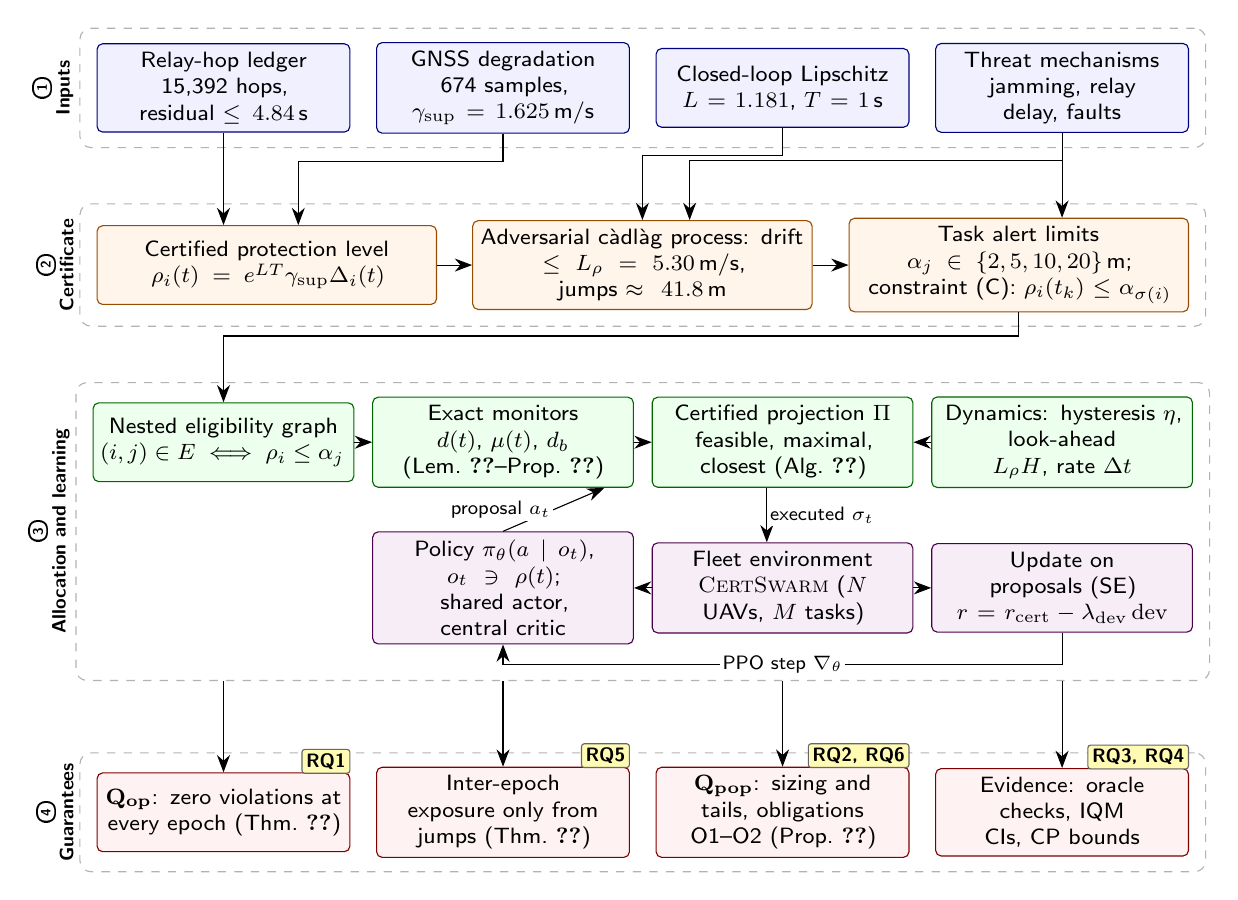
\begin{tikzpicture}[
  font=\sffamily\footnotesize,
  execute at begin node={\hyphenpenalty=10000\exhyphenpenalty=10000},
  >={Stealth[length=2.2mm]},
  box/.style={draw, rounded corners=2pt, align=center, minimum height=10mm,
              text width=#1, inner sep=3pt, fill=white},
  box/.default={31mm},
  data/.style={box=30mm, fill=blue!6, draw=blue!50!black},
  cert/.style={box=41mm, fill=orange!8, draw=orange!60!black},
  cons/.style={box=31mm, fill=green!7, draw=green!40!black},
  learn/.style={box=31mm, fill=violet!7, draw=violet!60!black},
  outb/.style={box=30mm, fill=red!5, draw=red!50!black},
  lane/.style={draw=black!30, dashed, rounded corners=4pt, inner xsep=6pt, inner ysep=5pt},
  lbl/.style={font=\sffamily\bfseries\scriptsize, rotate=90, anchor=south, inner sep=2pt, align=center},
  rq/.style={draw=black!60, fill=yellow!30, rounded corners=1pt, inner sep=1.5pt,
             font=\sffamily\scriptsize\bfseries},
  lab/.style={font=\sffamily\scriptsize, fill=white, inner sep=1pt}
]
% ================= band 1: measured inputs
\node[data] (hop) at (0,0)     {Relay-hop ledger\\ \nNHops\ hops, residual $\le\nHiddenMax$\,s};
\node[data] (gam) at (3.55,0)  {GNSS degradation\\ 674 samples, $\gamma_{\sup}=\nGammaSup$\,m/s};
\node[data] (lip) at (7.1,0)   {Closed-loop Lipschitz\\ $L=\nLloc$, $T=1$\,s};
\node[data] (thr) at (10.65,0) {Threat mechanisms\\ jamming, relay delay, faults};
\node[lane, fit=(hop)(gam)(lip)(thr)] (L1) {};
\node[lbl] at (L1.west) {\textcircled{\tiny 1}\\ Inputs};

% ================= band 2: certificate as constraint
\node[cert] (rho)  at (0.55,-2.25) {Certified protection level\\ $\rho_i(t)=e^{LT}\gamma_{\sup}\Delta_i(t)$};
\node[cert] (proc) at (5.32,-2.25) {Adversarial c\`adl\`ag process: drift\\ $\le L_\rho=\nKappa$\,m/s, jumps $\approx\nJumpMed$\,m};
\node[cert] (al)   at (10.1,-2.25) {Task alert limits $\alpha_j\in\{2,5,10,20\}$\,m;\\ constraint (C): $\rho_i(t_k)\le\alpha_{\sigma(i)}$};
\node[lane, fit=(rho)(proc)(al)] (L2) {};
\node[lbl] at (L2.west) {\textcircled{\tiny 2}\\ Certificate};

% ================= band 3: allocation and learning
\node[cons] (graph)  at (0,-4.5)     {Nested eligibility graph\\ $(i,j)\in E\iff\rho_i\le\alpha_j$};
\node[cons] (closed) at (3.55,-4.5)  {Exact monitors\\ $d(t)$, $\mu(t)$, $d_b$ (Lem.~\ref{lem:ore}--Prop.~\ref{prop:graded})};
\node[cons] (proj)   at (7.1,-4.5)   {Certified projection $\Pi$\\ feasible, maximal, closest (Alg.~\ref{alg:proj})};
\node[cons] (dyn)    at (10.65,-4.5) {Dynamics: hysteresis $\eta$,\\ look-ahead $L_\rho H$, rate $\Delta t$};
\node[learn] (pol)   at (3.55,-6.35) {Policy $\pi_\theta(a\mid o_t)$, $o_t\ni\rho(t)$;\\ shared actor, central critic};
\node[learn] (env)   at (7.1,-6.35)  {Fleet environment\\ \textsc{CertSwarm} ($N$ UAVs, $M$ tasks)};
\node[learn] (upd)   at (10.65,-6.35){Update on proposals (SE)\\ $r=r_{\mathrm{cert}}-\lambda_{\mathrm{dev}}\,\mathrm{dev}$};
\coordinate (loopbot) at (3.55,-7.35);
\node[lane, fit=(graph)(closed)(proj)(dyn)(pol)(env)(upd)(loopbot)] (L3) {};
\node[lbl] at (L3.west) {\textcircled{\tiny 3}\\ Allocation and learning};

% ================= band 4: guarantees and evaluation
\node[outb] (qop)  at (0,-9.2)     {$\mathbf{Q_{op}}$: zero violations at every epoch (Thm.~\ref{thm:proj})};
\node[outb] (exp)  at (3.55,-9.2)  {Inter-epoch exposure only from jumps (Thm.~\ref{thm:predict})};
\node[outb] (qpop) at (7.1,-9.2)   {$\mathbf{Q_{pop}}$: sizing and tails, obligations O1--O2 (Prop.~\ref{prop:lift})};
\node[outb] (ev)   at (10.65,-9.2) {Evidence: oracle checks, IQM CIs, CP bounds};
\node[lane, fit=(qop)(exp)(qpop)(ev)] (L4) {};
\node[lbl] at (L4.west) {\textcircled{\tiny 4}\\ Guarantees};

% ================= arrows
\draw[->] (hop.south) -- (hop.south |- rho.north);
\draw[->] (gam.south) -- ++(0,-0.35) -| ([xshift=4mm]rho.north);
\draw[->] (lip.south) -- ++(0,-0.35) -| (proc.north);
\draw[->] (thr.south) -- (thr.south |- al.north);
\draw[->] (thr.south) ++(0,-0.35) -| ([xshift=6mm]proc.north);
\draw[->] (rho) -- (proc);
\draw[->] (proc) -- (al);
\draw[->] (al.south) -- ++(0,-0.3) -| (graph.north);
\draw[->] (graph) -- (closed);
\draw[->] (closed) -- (proj);
\draw[->] (dyn) -- (proj);
\draw[->] (pol.north) -- node[lab, left]{proposal $a_t$} ([xshift=-6mm]proj.south west |- proj.south) ;
\draw[->] ([xshift=-2mm]proj.south) -- node[lab, right]{executed $\sigma_t$} ([xshift=-2mm]env.north);
\draw[->] (env) -- (upd);
\draw[->] (upd.south) -- ++(0,-0.4) -| node[lab, pos=0.25]{PPO step $\nabla_\theta$} (pol.south);
\draw[->] (env) -- (pol);
\draw[->] (L3.south -| qop) -- (qop.north);
\draw[->] (L3.south -| exp) -- (exp.north);
\draw[->] (L3.south -| qpop) -- (qpop.north);
\draw[->] (L3.south -| ev) -- (ev.north);

% ================= research-question tags
\node[rq, anchor=south east] at ([yshift=-0.5pt]qop.north east) {RQ1};
\node[rq, anchor=south east] at ([yshift=-0.5pt]exp.north east) {RQ5};
\node[rq, anchor=south east] at ([yshift=-0.5pt]qpop.north east) {RQ2, RQ6};
\node[rq, anchor=south east] at ([yshift=-0.5pt]ev.north east) {RQ3, RQ4};
\end{tikzpicture}}
\caption{Methodological framework, read top to bottom. \textcircled{\scriptsize 1}~Measured
quantities from the parent artifact determine \textcircled{\scriptsize 2}~each aircraft's
certified protection level $\rho_i(t)$, a bounded c\`adl\`ag process that drifts under
jamming and jumps under relay delay; a task may be held only while $\rho_i(t)$ does not
exceed its alert limit $\alpha_j$. \textcircled{\scriptsize 3}~Because the constraint is a
scalar threshold on each side, the eligibility graph is nested. Closed forms monitor the
coverage the fleet can certify, and a projection inside the environment maps every proposal
of the learning policy to a feasible, coverage-maximal assignment, so training never executes
an infeasible one. \textcircled{\scriptsize 4}~The outputs are a per-operation guarantee and
a population statement whose assumptions are listed as evidence obligations. Tags give the
research question that each output answers.}
\label{fig:framework}
\end{figure}

\FloatBarrier

% =====================================================================
\section{Methodology I: Certified Allocation under Nested Constraints}
\label{sec:theory}
% =====================================================================
Proofs are in \cref{app:proofs}. Throughout, $d(t)$, $n_k(t)$ and $G(t)$ are evaluated at
the current certificates. We drop $t$ when no confusion arises.

\subsection{Exact monitors}
\begin{lemma}[Certified coverage; Ore~\cite{ore1955} on nested graphs]
\label{lem:ore}
The maximum number of tasks coverable by a feasible assignment is $M-d$, where
\begin{equation}
\label{eq:deficiency}
d\;=\;\max_{1\le k\le M}\bigl(k-n_k\bigr)^{+}.
\end{equation}
It is computable in $O(N\log N+M\log M)$, and a maximum feasible assignment is produced by
processing tasks in ascending $\alpha$ and giving each one \emph{any} still-free eligible
aircraft.
\end{lemma}

\begin{lemma}[Coverage margin; $b$-extended Hall~\cite{laroche2014interdiction}]
\label{lem:margin}
Full coverage survives the collapse ($\rho\to\infty$) of \emph{any} $b$ aircraft iff
$n_k\ge k+b$ for all $k$. The largest such $b$ is the \emph{coverage margin}
$\mu=\min_k(n_k-k)$, and full coverage currently fails iff $\mu<0$.
\end{lemma}

The margin is a procurement quantity. It counts the simultaneous certificate failures that
the fleet absorbs with no loss of coverage. The next two results give the exact worst case
when that budget is exceeded.

\begin{proposition}[Optimal collapse adversary]
\label{prop:collapse}
If an adversary may collapse any $b$ certificates, the maximum certified coverage
afterwards is $M-d_b$ with $d_b=\max_k\bigl(k-(n_k-b)^{+}\bigr)^{+}$. The minimum is
attained by collapsing the $b$ aircraft with the smallest $\rho$.
\end{proposition}

\begin{proposition}[Graded degradation, exact worst case]
\label{prop:graded}
Let any $b$ aircraft have their protection level increased by $s\ge0$, for example by $s/\Lrho$
seconds of dead reckoning. Let $n^{(s)}_k=|\{i:\rho_i+s\le\alpha_{(k)}\}|$. Then the
maximum certified coverage afterwards is at least
\begin{equation}
\label{eq:graded}
M-\max_k\bigl(k-\max\{\,n_k-b,\;n^{(s)}_k\}\bigr)^{+},
\end{equation}
and an adversary choosing the $b$ aircraft attains this value. As $s\to\infty$ it reduces to
\cref{prop:collapse}.
\end{proposition}

The generic bound ``each failure costs at most one task'', $M-d-b$, is valid but loose.
\Cref{prop:collapse,prop:graded} are exact, and on our fleets the gap is several tasks
(\cref{sec:rq2}). Classical coverage control treats failed agents as
binary~\cite{cortes2004coverage}. Resilient multi-robot planning bounds submodular utility
after $\alpha$ worst-case removals~\cite{zhou2019resilienttracking,zhou2022attackrobust}.
\Cref{prop:graded} is exact for graded degradation, which is what jamming produces.

\subsection{The certified projection layer}
The projection sits in the environment: the policy proposes, the environment executes
$\Proj$ of the proposal, and the policy is trained on what it proposed. Following
\citet{markgraf2025actionprojection}, we call this the \emph{safeguard-in-environment} (SE)
placement, as opposed to placing the safeguard inside the policy.

\begin{algorithm}[t]
\caption{Certified projection $\Proj$ (executed at every decision epoch)}
\label{alg:proj}
\begin{algorithmic}[1]
\Require proposal $a\in(\T\cup\{\idle\})^N$, certificates $\rho$, alert limits $\alpha$, values $v$, previous assignment $\sigma^-$
\Require band $\eta\in[0,1)$, $h\ge0$; look-aheads $\ell_{\mathrm{acq}},\ell_{\mathrm{keep}}\ge0$
\State $E_{ij}\gets\bigl[\rho_i+\ell_{\mathrm{acq}}\le(1-\eta)\alpha_j-h\bigr]$ for $j\ne\sigma^-(i)$;\quad $E_{i\sigma^-(i)}\gets\bigl[\rho_i+\ell_{\mathrm{keep}}\le\alpha_{\sigma^-(i)}\bigr]$ \Comment{acquire / keep}
\State $W_{ij}\gets B+c_v v_j+\mathbb 1[a_i=j]$ on $E$ \Comment{$c_v=(N+1)/\min\Delta v$, $B>M(c_v\max v+1)$}
\State $\sigma\gets$ maximum-weight matching of $(E,W)$ \Comment{Hungarian; greedy nested variant: \cref{lem:ore}}
\State \Return $\sigma$ \Comment{executed; the policy is trained on $a$ (SE placement)}
\end{algorithmic}
\end{algorithm}

\begin{theorem}[Certified projection]
\label{thm:proj}
Let $\Proj$ be \cref{alg:proj} with $\eta=h=\ell_{\mathrm{acq}}=\ell_{\mathrm{keep}}=0$.
For every policy $\pi_\theta$, every parameter value $\theta$ and every certificate
trajectory permitted by \cref{as:sound}, the executed assignment
$\sigma_{t_k}=\Proj(a_{t_k};s_{t_k})$ has the following properties:
\begin{enumerate}[label=(\roman*),leftmargin=1.8em,itemsep=0pt,topsep=1pt]
\item it satisfies (C) at every epoch of every episode, in training and in deployment;
\item it assigns exactly $M-d(t_k)$ tasks, the maximum. Among maximum assignments it
  maximises assigned value, where $\min\Delta v$ is the smallest gap between distinct task
  values; among those it maximises agreement with the proposal $a_{t_k}$;
\item if, in addition, the threat process is Markov in a state $s$ that includes $\sigma^-$,
  the process seen by the policy is a Markov decision process (MDP) with kernel
  $P_\Proj(s'\mid s,a)=P(s'\mid s,\Proj(a;s))$. Its observations are partial when the
  policy is decentralised. The likelihood-ratio policy gradient of the projected objective is
  therefore unbiased, and PPO incurs no bias beyond its usual clipping and critic bias.
  Differentiating through $\Proj$ instead gives zero gradient almost everywhere, because
  $\Proj$ is piecewise constant in $a$.
\end{enumerate}
For the coverage-only objective, the greedy nested variant of \cref{lem:ore} achieves (i)
and the cardinality part of (ii) in $O(N\log N+M\log M)$.
\end{theorem}

Two remarks place \cref{thm:proj}. First, part (i) alone is easy: the constraint is
separable across aircraft, so per-agent action masking~\cite{huang2022masking,boutilier2018sas}
also never violates it. Theorem~\ref{thm:proj}(i) is then the familiar shield guarantee,
transposed to a certificate-driven set. What masking cannot provide is (ii). Agents that each pick a
feasible task still collide, leaving coverage below $M-d$; \cref{sec:rq3} measures the
difference. Second, the placement in (iii) follows the safeguard-in-environment analysis
of~\cite{markgraf2025actionprojection}. That analysis shows that action aliasing, where many
proposals map to one executed action, harms policy gradients more when the safeguard sits in
the policy. Our setting has a further adversarial component: under \cref{as:sound} alone, the
projected process is a game against the jammer rather than an MDP, and (i)--(ii) still hold
while (iii) does not. We add a small penalty $\lambda_{\mathrm{dev}}$ on the fraction of proposals the
projection overrides, so the policy learns to propose assignments the projection keeps.

\subsection{Dynamics between and across epochs}
Constraint (C) binds at decision epochs. Between epochs the certificate keeps moving, and
across epochs an aircraft whose $\rho_i$ hovers near $\alpha_j$ could acquire and drop a
task repeatedly. We call a holder \emph{exposed} on $[t_k,t_{k+1})$ if (C) held at $t_k$
and fails before $t_{k+1}$. A \emph{forced release} occurs when a holder becomes
ineligible for its own task. Let $\TVp_i[0,\tau]$ be the positive variation of $\rho_i$ on
$[0,\tau]$: the sum of all its increases, including jumps.

\begin{theorem}[Hysteresis]
\label{thm:hyst}
With band $(\eta,h)$ in \cref{alg:proj} and $\ell_{\mathrm{keep}}=0$, the number of forced
releases of aircraft $i$ on $[0,\tau]$ is at most
$1+\TVp_i[0,\tau]/(\eta\alpha_{(1)}+h)$. If
$\ell_{\mathrm{keep}}\le\ell_{\mathrm{acq}}+h$, the number of assigned feasible tasks is at
least $M-d(\tilde\rho)$, where $\tilde\rho_i=(\rho_i+h+\ell_{\mathrm{acq}})/(1-\eta)$.
\end{theorem}

\begin{theorem}[Predictive feasibility and the allocator rate]
\label{thm:predict}
Suppose that between upward jumps every $\rho_i$ grows at rate at most $\Lrho$. If
$\ell_{\mathrm{keep}}\ge\Lrho\Delta t$ and $\ell_{\mathrm{acq}}\ge\Lrho H$ with $H\ge\Delta t$,
then:
\begin{enumerate}[label=(\roman*),leftmargin=1.8em,itemsep=0pt,topsep=1pt]
\item a holder can be exposed on $[t_k,t_{k+1})$ only if its certificate jumps upward in
  that interval, so the number of exposed holder-epochs is at most the number of upward
  jumps;
\item a newly acquired task remains feasible for at least $H$ unless a jump occurs.
\end{enumerate}
An aircraft whose protection level is $\rho$ can hold a task with alert limit $\alpha$
under this rule only if $\Delta t\le(\alpha-\rho)/\Lrho$.
\end{theorem}

With the measured constants, an aircraft at the benign ceiling
$\bar\rho_0=\nRhoFloor$\,m can hold a $\nAlphaMin$\,m corridor only if
$\Delta t\le(\nAlphaMin-\nRhoFloor)/\nKappa=\nDtMax$\,s. This is the allocator rate of
$\nRateMin$\,Hz quoted in the abstract: the rate at which \emph{every} benign aircraft
remains usable for the most demanding task. Aircraft with a lower benign level tolerate
slower rates. \Cref{sec:rq5} tests the rule at 2\,Hz and at 5.3\,Hz. Jumps cannot be
predicted from a rate bound: a stale correction arrives all at once. \Cref{thm:predict}
therefore isolates exactly what prediction can and cannot remove.

\begin{proposition}[Misreported certificates]
\label{prop:liars}
If $f$ aircraft report a protection level other than their true one, the reported deficiency
differs from the true one by at most $f$. Moreover, every violation of (C) under $\Proj$ is
committed by a misreporting aircraft.
\end{proposition}

The deficiency depends on the certificates only through the count profile $(n_k)$, which
needs one counter per alert-limit class. Counts can be agreed in a decentralised fleet by
resilient consensus~\cite{leblanc2013wmsr}. Authenticated certificate reports, whose cost is budgeted
in~\cite{paperI}, reduce $f$ to the number of compromised signing keys.

\subsection{From one operation to a population}
\label{sec:lift}
\Cref{thm:proj} is a $\Qop$ statement: it holds surely for one operation, given
\cref{as:sound}. Fleet sizing and per-flight-hour objectives need $\Qpop$ statements, such
as the probability that a fleet of size $N$ covers every task at a random instant of a
random operation. The companion systematisation shows that no chain of proofs alone reaches
such an objective: every path crosses a statistical obligation~\cite{paperII}. The lift below names its own
obligations.

\begin{proposition}[Population lift]
\label{prop:lift}
Group the alert limits into classes $\lambda_1<\dots<\lambda_c$ with $m_\ell$ tasks at or
below $\lambda_\ell$. Assume two obligations:
\begin{itemize}[leftmargin=2.6em,itemsep=0pt,topsep=1pt]
\item[\textbf{O1}] at a random instant, and conditionally on the task set, the aircraft's
  classes $\ell_i=\min\{\ell:\rho_i\le\lambda_\ell\}$ (with $\ell_i=c+1$, ``none'', if
  $\rho_i>\lambda_c$) are independent across aircraft;
\item[\textbf{O2}] the classes are identically distributed with law $q$, with $q$ estimated
  from operations representative of deployment.
\end{itemize}
Then
\[
\Prob\bigl(d=0\bigr)=\Prob\Bigl(\textstyle\sum_{\ell'\le\ell}C_{\ell'}\ge m_\ell\ \ \forall\ell\Bigr),
\]
where $C\sim\mathrm{Multinomial}(N,q)$ over the $c+1$ classes; this is computable exactly by dynamic programming in
$O(cN^2)$. The smallest fleet $N^\star(\delta)$ with $\Prob(d=0)\ge1-\delta$ is the
fleet-sizing answer, and the deficiency tail $\Prob(d\ge k)$ follows the same way.
\end{proposition}

O1 is precisely what a common-cause failure breaks. One jammer degrades every aircraft in
its footprint at once. \Cref{sec:rq6} shows that the independent model then
\emph{underestimates} multi-task loss, the operationally dangerous direction. Whenever zero
violations are observed over $n$ agent-epochs, we report the exact one-sided 95\%
Clopper--Pearson (CP) upper bound on the per-epoch violation rate~\cite{clopper1934}. It is
approximately $3/n$, the ``rule of three''~\cite{hanley1983ruleofthree} that also underlies
the test-hour ladders of the Specific Operations Risk Assessment (SORA)~\cite{jarus2019sora,paperII}.

\begin{remark}[Where the closed forms stop]
\label{rem:frontier}
Nestedness needs a scalar certificate against a scalar alert limit. With vector certificates
(horizontal and vertical protection levels, link quality), eligibility becomes a dominance
order. Maximum matching remains polynomial~\cite{hopcroft1973}, but \cref{eq:deficiency}
and the linear-time monitors are lost. Robust assignment under vertex failures is then hard
to approximate in general~\cite{adjiashvili2017vulnerable}. The scalar case is therefore the
largest one in which every monitor is a closed form.
\end{remark}

% =====================================================================
\section{Methodology II: Experimental Design}
\label{sec:design}
% =====================================================================
\paragraph{Certificate process.} We generate $\rho_i(t)$ by \eqref{eq:rho} from three
independent mechanisms per aircraft:
\begin{itemize}[leftmargin=1.2em,itemsep=0pt,topsep=1pt]
\item dead reckoning under jamming or sensor faults: staleness grows at 1\,s/s, Poisson
  onsets, exponential durations, and a 2\,s re-anchoring delay;
\item undetected relay-delay episodes over $H=2$ hops: staleness jumps by the sum of two
  residuals drawn from the \nNHidden\ measured undetected residuals;
\item a benign floor drawn from the \nNBenign\ measured benign residuals.
\end{itemize}
Spatial jammers (radius 200\,m, random walk) add common-cause dead reckoning to every
aircraft in their footprint. Rates are stated modelling assumptions and are swept; every
magnitude is measured. \Cref{app:constants} lists each constant with its provenance.

\paragraph{Environment.} \textsc{CertSwarm} is a vectorised environment of $B$ fleets with
$N=12$ aircraft and $M=8$ tasks on a $1\times1$\,km arena. Aircraft fly at 15\,m/s, and a
task is on site within 30\,m. Two spatial jammers roam the arena. Decision epochs are $\Delta t=0.5$\,s, and missions last
150\,s. Alert limits are drawn from $\{2,5,10,20\}$\,m with values $\{4,3,2,1\}$.

Each aircraft observes:
\begin{itemize}[leftmargin=1.2em,itemsep=0pt,topsep=1pt]
\item its own position, $\rho_i$, the change in $\rho_i$, and whether it holds a task;
\item for each task, in egocentric order of distance: relative position, alert limit,
  value, eligibility, and whether it or another aircraft holds the task;
\item the fleet's count profile and the jammer offsets.
\end{itemize}
The jamming-blind variant zeroes every certificate-derived feature.

\paragraph{Learning.} We use proximal policy optimisation (PPO)~\cite{schulman2017ppo} in
the multi-agent PPO (MAPPO) style~\cite{yu2022mappo}. A parameter-shared actor outputs, per
aircraft, a categorical over \{keep, idle, $k$-th nearest task\}. A centralised critic sees
the aircraft's observation and the fleet mean. Training uses 16 parallel fleets, rollouts of
150 epochs and 200 updates (480k fleet-epochs, $5.8\times10^6$ agent-epochs per run), with
\nNSeeds\ training seeds per method. \Cref{app:hyper} lists all hyperparameters.

\paragraph{Methods.}
\begin{itemize}[leftmargin=1.2em,itemsep=1pt,topsep=1pt]
\item \emph{Ours}: \cref{alg:proj} in the environment, reward $\rcert$, and deviation
  penalty $\lambda_{\mathrm{dev}}=0.05$. The ablation sets $\lambda_{\mathrm{dev}}=0$.
\item \emph{Masking}: invalid-action masking per aircraft~\cite{huang2022masking}, with
  conflicts resolved by the first claimant.
\item \emph{PPO-Lagrangian}~\cite{ray2019safetygym,stooke2020pid}: the certificate is
  observed but not enforced. The reward is nominal coverage minus $\lambda$ times the
  violation rate; $\lambda$ is updated by dual ascent to a limit of 0.5\% violating
  agent-epochs.
\item \emph{Jamming-blind PPO}: no certificate features, nominal reward.
\item Every learned policy without the layer is also evaluated \emph{with the projection
  added at deployment}, separating what the policy learns from what the mechanism
  enforces.
\item Non-learned references:
  \begin{itemize}[leftmargin=1em,itemsep=0pt,topsep=0pt]
  \item keep-or-nearest proposals with the projection;
  \item the tightest-fit greedy allocator re-solved every epoch;
  \item a fixed design margin that admits task $j$ iff
    $\rho_0+\Lrho\cdot1\,\mathrm{s}\le\alpha_j$, i.e.\ one second of dead reckoning
    budgeted at design time;
  \item keep-or-nearest with no certificate.
  \end{itemize}
\end{itemize}

\paragraph{Metrics and statistics.} We report:
\begin{itemize}[leftmargin=1.2em,itemsep=0pt,topsep=1pt]
\item certified coverage $\rcert$;
\item the \emph{coverage ratio}, feasible holders over the maximum $M-d(t)$ from
  \cref{lem:ore}, which separates ``safe because idle'' from ``safe and maximal'';
\item violations per agent-epoch, counted per step and never averaged over episodes, in
  training and in evaluation;
\item inter-epoch exposure and reassignments per agent-epoch.
\end{itemize}
Each learned method is evaluated greedily on 3 held-out seeds $\times$ 16 fleets per training
seed. We report the interquartile mean (IQM) with 95\% stratified-bootstrap confidence
intervals (CIs)~\cite{agarwal2021precipice}, and CP bounds whenever zero violations are
observed.

% =====================================================================
\section{Results}
\label{sec:results}
% =====================================================================
\subsection{Correctness of the closed forms}
Over \nVerInst\ random nested instances (up to 10 aircraft and 10 tasks, with ties,
continuous and heavy-tailed certificates), we compared every closed form with a
brute-force oracle: Hopcroft--Karp matching~\cite{hopcroft1973}, enumeration of all
$b$-subsets, and enumeration of task subsets for value. The checks covered:
\begin{itemize}[leftmargin=1.2em,itemsep=0pt,topsep=1pt]
\item \cref{lem:ore}, the greedy and lexicographic projections, and value optimality;
\item \cref{lem:margin} and \cref{prop:collapse};
\item the coverage bound of \cref{thm:hyst}.
\end{itemize}
The \nVerChecks\ checks total \nVerTotal\ comparisons with \nVerDisagree\ disagreements. A
further \nLiarInst\ instances per misreporting level confirm \cref{prop:liars}: no honest
aircraft ever violated (C). This is a check on the mathematics and the implementation, not
evidence about flight.

% RQ1 and RQ3: the multi-agent learning study. Numbers from numbers.tex / tab_main.tex.
\subsection{RQ1: violations during learning}
\label{sec:rq1}
\Cref{fig:training} tracks certified coverage and cumulative violations over training.
\begin{itemize}[leftmargin=1.2em,itemsep=1pt,topsep=1pt]
\item \emph{Projection in the environment.} It executed \emph{zero} infeasible assignments
  over $\nOursTrainSteps$ agent-epochs, pooled across \nNSeeds\ seeds, from the first update
  onwards. Per-agent masking also reached zero, as separability predicts. For both methods
  zero holds by construction, so the CP bound in \cref{tab:main} only quantifies the
  exposure observed. That bound assumes independent agent-epochs, which these are not.
\item \emph{PPO-Lagrangian.} Although it observes the certificate, it executed
  \nLagTrainViol\ infeasible assignments while learning, $\nLagTrainRate\%$ of agent-epochs.
  Its multiplier then rose until the policy largely stopped serving tasks. Final certified
  coverage is $\nLagCov$, and evaluation violations still average $\nLagViolMean\%$ of
  agent-epochs, above the 0.5\% limit.
\item \emph{Jamming-blind PPO.} It executed \nBlindTrainViol\ infeasible assignments
  ($\nBlindTrainRate\%$).
\item \emph{Stronger in-expectation learners} (\cref{tab:r2}). MAPPO-Lagrangian with a cost
  critic executed \nMLagTrainViol\ infeasible assignments while learning
  ($\nMLagTrainRate\%$), and \nMLagZeroTrainViol\ with a cost limit of zero.
  PID-Lagrangian executed \nPidLagTrainViol\ and then stopped serving tasks altogether.
  QMIX without masks executed \nQmixTrainViol. Only the two methods that remove infeasible
  actions by construction, our layer and masking (with PPO or with QMIX), learned without a
  violation.
\end{itemize}
In-expectation methods violate the constraint while they learn, and learning is when a
fleet would be flight-tested. No setting of the Lagrangian's cost limit or dual step changed
this (\cref{app:sens}).

\begin{figure*}[t]
\centering
\begin{tikzpicture}
\begin{groupplot}[group style={group size=2 by 1, horizontal sep=1.4cm},
  width=0.46\textwidth, height=4.2cm, xlabel={fleet-epochs ($\times10^3$)},
  grid=major, grid style={black!10}, tick label style={font=\scriptsize},
  label style={font=\small}, xmin=0, xmax=480,
  legend style={font=\scriptsize, fill=white, fill opacity=0.85, text opacity=1}]
\nextgroupplot[ylabel={certified coverage $r_{\mathrm{cert}}$}, ymin=0, ymax=0.8,
  legend style={at={(0.98,0.98)}, anchor=north east, font=\tiny}, legend columns=2]
\addplot[name path=ou, draw=none, forget plot] table[x=steps,y=hi]{figdata/curve_ours.dat};
\addplot[name path=ol, draw=none, forget plot] table[x=steps,y=lo]{figdata/curve_ours.dat};
\addplot[red!20, forget plot] fill between[of=ou and ol];
\addplot[red!70!black, thick] table[x=steps,y=rcert]{figdata/curve_ours.dat};
\addplot[orange!80!black, thick] table[x=steps,y=rcert]{figdata/curve_mask.dat};
\addplot[blue!70!black, thick] table[x=steps,y=rcert]{figdata/curve_lagrangian.dat};
\addplot[gray, thick, dashed] table[x=steps,y=rcert]{figdata/curve_blind.dat};
\legend{projection (ours), masking, PPO-Lagrangian, jamming-blind}
\nextgroupplot[ylabel={cumulative violations (mean per run)}, ymode=log, ymin=0.8, ymax=3e6,
  legend pos=south east]
\addplot[red!70!black, thick] table[x=steps,y=cumviol]{figdata/curve_ours.dat};
\addplot[orange!80!black, thick, densely dotted] table[x=steps,y=cumviol]{figdata/curve_mask.dat};
\addplot[blue!70!black, thick] table[x=steps,y=cumviol]{figdata/curve_lagrangian.dat};
\addplot[gray, thick, dashed] table[x=steps,y=cumviol]{figdata/curve_blind.dat};
\legend{projection (0), masking (0), PPO-Lagrangian, jamming-blind}
\end{groupplot}
\end{tikzpicture}
\caption{RQ1. Left: certified coverage during training (stochastic policy; mean over
\nNSeeds\ seeds, 10-update moving average; band: min--max across seeds for ours). Right: cumulative executed
violations on a log axis. Zero is drawn at 1 for visibility. The projection and masking
curves lie on the floor throughout.}
\label{fig:training}
\end{figure*}

\subsection{RQ3: what the policy learns and what the mechanism enforces}
\label{sec:rq3}
\Cref{tab:main} evaluates every method greedily on held-out missions. Four findings stand out.

\emph{The mechanism does most of the work.} Adding the projection at deployment to \emph{any}
learned policy removed every violation and lifted the coverage ratio to at least
$\nLagProjRatio$:
\begin{itemize}[leftmargin=1.2em,itemsep=0pt,topsep=1pt]
\item jamming-blind: certified coverage $\nBlindCov\to\nBlindProjCov$;
\item masking: $\nMaskCov\to\nMaskProjCov$;
\item PPO-Lagrangian: $\nLagCov\to\nLagProjCov$.
\end{itemize}
Without it, the jamming-blind policy and the no-certificate heuristic reach seemingly
competitive certified coverage ($\nBlindCov$ and $\nHeurNoneCov$). They do so only by holding
tasks without certification on $\nBlindViolMean\%$ and $\nHeurNoneViolMean\%$ of
agent-epochs. The jamming-blind policy in fact converges to the keep-or-nearest rule, with no
reassignments.

\emph{Masking is safe but not maximal.} Its coverage ratio of $\nMaskRatio$ is the gap that
\cref{thm:proj}(ii) closes. Agents that each pick an eligible task still collide.

\emph{Learning adds little on top of the guarantee, and where the layer sits during training
does not matter.}
\begin{itemize}[leftmargin=1.2em,itemsep=0pt,topsep=1pt]
\item The policy trained with the projection reaches $\nOursCov$ [$\nOursCovLo$,
  $\nOursCovHi$] at a coverage ratio of $\nOursRatio$, over \nNSeeds\ training seeds.
\item The keep-or-nearest heuristic with the same projection reaches $\nHeurCov$; the
  intervals only just separate.
\item Policies trained with masking, or blind, and projected at deployment do as well
  ($\nMaskProjCov$, $\nBlindProjCov$), and the deviation penalty makes no measurable
  difference ($\nNoDevCov$ without it).
\end{itemize}
What training \emph{with} the projection buys is the zero-violation learning of RQ1, not a
better final policy.

\emph{Static and design-time allocators fail in opposite ways.} The tightest-fit greedy
re-solves from scratch every epoch, keeps its aircraft in transit ($\nGnpSwitch\%$
reassignments) and certifies only $\nGnpCov$. A fixed design margin certifies $\nFixedCov$
and still violates on $\nFixedViolMean\%$ of agent-epochs, because a margin fixed at design
time cannot track a certificate that moves.

\begin{table*}[t]
\centering\footnotesize
\setlength{\tabcolsep}{3.5pt}
\caption{RQ3. Held-out evaluation ($N=12$, $M=8$; \nNSeeds\ training seeds $\times$ 3
evaluation seeds $\times$ 16 fleets for learned methods; 3 $\times$ 16 for the references
below the line). Values are IQMs with 95\% stratified-bootstrap CIs. Cov.\ ratio: feasible
holders divided by $(M-d)$. Violations are in \% of agent-epochs (IQM over runs). ``$0\,(\le
x)$'': none observed, with the 95\% CP upper bound on the rate, assuming independent
agent-epochs. Train viol.: executed infeasible assignments over all of training.}
\label{tab:main}
\resizebox{\linewidth}{!}{%
\begin{tabular}{@{}lcccccc@{}}
\toprule
Method & $r_{\mathrm{cert}}$ & cov.\ ratio & eval viol. [\%] & train viol. & exposure [\%] & reassign. [\%]\\
\midrule
\textbf{Projection (SE) + PPO (ours)} & $0.496$ {\scriptsize[0.473, 0.525]} & $1.00$ & $0$ ($\le3.5\times10^{-6}$) & $0$ ($\le1.0\times10^{-7}$) & $1.62$ & $4.9$ \\
\quad ablation: no deviation penalty & $0.499$ {\scriptsize[0.484, 0.520]} & $1.00$ & $0$ ($\le3.5\times10^{-6}$) & $0$ ($\le1.0\times10^{-7}$) & $1.66$ & $4.9$ \\
Per-agent action masking + PPO & $0.464$ {\scriptsize[0.458, 0.473]} & $0.62$ & $0$ ($\le3.5\times10^{-6}$) & $0$ ($\le1.0\times10^{-7}$) & $0.52$ & $0.7$ \\
\quad + projection at deployment & $0.499$ {\scriptsize[0.489, 0.508]} & $1.00$ & $0$ ($\le3.5\times10^{-6}$) & -- & $1.71$ & $4.9$ \\
PPO-Lagrangian (certificate observed) & $0.036$ {\scriptsize[0.028, 0.047]} & $0.04$ & $0.02$ & $3{,}903{,}179$ & $0.03$ & $0.0$ \\
\quad + projection at deployment & $0.393$ {\scriptsize[0.383, 0.405]} & $0.99$ & $0$ ($\le3.5\times10^{-6}$) & -- & $1.48$ & $3.9$ \\
Jamming-blind PPO & $0.451$ {\scriptsize[0.439, 0.467]} & $0.51$ & $13.75$ & $4{,}744{,}505$ & $0.37$ & $0.0$ \\
\quad + projection at deployment & $0.492$ {\scriptsize[0.478, 0.508]} & $1.00$ & $0$ ($\le3.5\times10^{-6}$) & -- & $1.71$ & $5.0$ \\
\midrule
Keep-or-nearest + projection & $0.435$ {\scriptsize[0.395, 0.477]} & $1.00$ & $0$ ($\le1.7\times10^{-5}$) & -- & $1.45$ & $2.3$ \\
Tightest-fit greedy, re-solved each epoch & $0.169$ {\scriptsize[0.142, 0.216]} & $0.98$ & $0$ ($\le1.7\times10^{-5}$) & -- & $1.99$ & $8.6$ \\
Fixed design margin (1\,s dead reckoning) & $0.163$ {\scriptsize[0.155, 0.170]} & $0.31$ & $8.03$ & -- & $0.20$ & $0.0$ \\
Keep-or-nearest, no certificate & $0.459$ {\scriptsize[0.433, 0.484]} & $0.51$ & $13.97$ & -- & $0.38$ & $0.0$ \\
\bottomrule
\end{tabular}}

\end{table*}

\subsection{RQ3 (continued): stronger baselines and a classical auction}
\label{sec:rq3b}
\Cref{tab:r2} adds the stronger learners and a non-learned consensus auction at the
headline size. Three findings matter for the security argument.

\emph{Better in-expectation learners still violate, and the monitor still repairs them.}
MAPPO-Lagrangian with a cost critic is the strongest unconstrained learner: it reaches
$\nMLagCov$ certified coverage and, once trained, violates on only $\nMLagEvalViolPct\%$ of
agent-epochs. Its guarantee is nonetheless in expectation: it paid for that policy with
\nMLagTrainViol\ violations during learning, and lowering its cost limit to zero did not
remove them. With the projection at deployment, every learned policy in the table executes
no violation and reaches a coverage ratio of at least $\nProjMinRatio$.

\emph{A classical auction under the same constraint beats every learned allocator.} CBBA
with feasibility enforced inside the bundle certifies $\nCbbaCov$ [$\nCbbaCovLo$,
$\nCbbaCovHi$] of the task value, against $\nOursCov$ [$\nOursCovLo$, $\nOursCovHi$] for the
best learned policy, with no violation and a coverage ratio of $\nCbbaRatio$. The comparison
favours the auction in one respect: its consensus phase gives every aircraft the fleet's full
state at every epoch, while the learned policies act on local observations in one shot. In
our setting, that information is worth more than learning.

\emph{The result supports the paper's claim, not a learning claim.} Our guarantees do not
depend on which allocator proposes: they hold for the auction, for the heuristic, for every
learned policy and for an adversarially chosen one (A4). The learning study shows that the
monitor can sit in the training loop at no cost to learning; it does not show that learning
is the best allocator, and we do not claim it.

\begin{table}[t]
\centering\footnotesize
\setlength{\tabcolsep}{2.5pt}
\caption{RQ3. Stronger baselines at $N=12$ (\nMLagSeeds\ training seeds $\times$ 3
evaluation seeds $\times$ 16 fleets; CBBA is deterministic, 3 $\times$ 16). Columns as in
\cref{tab:main}; eval.\ violations in \% of agent-epochs.}
\label{tab:r2}
\resizebox{\columnwidth}{!}{\begin{tabular}{@{}lcccc@{}}
\toprule
Method & $r_{\mathrm{cert}}$ & cov.\ ratio & eval viol. [\%] & train viol.\\
\midrule
\textbf{Projection (SE) + PPO (ours)} & $0.491$ {\scriptsize[0.477, 0.509]} & $1.00$ & $0$ ($\le1.7\times10^{-6}$) & $0$ ($\le5.2\times10^{-8}$) \\
Keep-or-nearest + projection & $0.435$ {\scriptsize[0.395, 0.477]} & $1.00$ & $0$ ($\le1.7\times10^{-5}$) & -- \\
\midrule
MAPPO-Lagrangian, cost critic, limit $0.005$ & $0.445$ {\scriptsize[0.438, 0.451]} & $0.57$ & $0.027$ & $2{,}897{,}602$ \\
\quad + projection at deployment & $0.463$ {\scriptsize[0.455, 0.473]} & $0.99$ & $0$ ($\le1.7\times10^{-6}$) & -- \\
MAPPO-Lagrangian, cost critic, limit $0$ & $0.442$ {\scriptsize[0.436, 0.451]} & $0.57$ & $0.091$ & $2{,}929{,}578$ \\
\quad + projection at deployment & $0.466$ {\scriptsize[0.455, 0.477]} & $1.00$ & $0$ ($\le1.7\times10^{-6}$) & -- \\
PID-Lagrangian PPO & $0.000$ {\scriptsize[0.000, 0.000]} & $0.00$ & $0.040$ & $8{,}089{,}556$ \\
\quad + projection at deployment & $0.347$ {\scriptsize[0.336, 0.360]} & $0.98$ & $0$ ($\le1.7\times10^{-6}$) & -- \\
QMIX (certificate observed) & $0.422$ {\scriptsize[0.410, 0.436]} & $0.60$ & $8.473$ & $7{,}526{,}523$ \\
\quad + projection at deployment & $0.460$ {\scriptsize[0.446, 0.477]} & $1.00$ & $0$ ($\le1.7\times10^{-6}$) & -- \\
QMIX with eligibility masks & $0.451$ {\scriptsize[0.444, 0.459]} & $0.68$ & $0$ ($\le1.7\times10^{-6}$) & $0$ ($\le5.2\times10^{-8}$) \\
\quad + projection at deployment & $0.455$ {\scriptsize[0.437, 0.473]} & $1.00$ & $0$ ($\le1.7\times10^{-6}$) & -- \\
CBBA, feasibility in the bundle & $0.539$ {\scriptsize[0.525, 0.561]} & $1.00$ & $0$ ($\le1.7\times10^{-5}$) & -- \\
\bottomrule
\end{tabular}
}
\end{table}

\subsection{RQ3 (continued): fleet size}
\label{sec:rq3c}
\Cref{tab:scale,fig:scale} repeat the core methods at $N\in\{\nScaleSizes\}$.
\begin{itemize}[leftmargin=1.2em,itemsep=1pt,topsep=1pt]
\item \emph{The guarantees scale.} Our layer and masking executed no infeasible assignment
  during training at any size, and our coverage ratio was at least $\nScaleMinRatio$
  throughout. PPO-Lagrangian executed millions of violations at every size and, from
  $N=24$ on, converged to idling ($\nScaleTwentyFourLag$ certified coverage).
\item \emph{Learning does not scale with our budget.} Certified coverage of the learned
  policy fell from $\nScaleTwelveOurs$ at $N=12$ to $\nScaleFortyEightOurs$ at $N=48$, with
  masking plus projection matching it at every size. It stayed above keep-or-nearest plus
  projection, separated at $N=\nScaleBeatsHeur$ and within the confidence intervals elsewhere.
\item \emph{The auction does.} CBBA certified $\nScaleTwelveCbba$, $\nScaleTwentyFourCbba$ and
  $\nScaleFortyEightCbba$ of the task value at the three sizes.
\end{itemize}
Our budget per size was 200 updates on 4 CPU cores, below the runbook's 400--600; larger
budgets may narrow the gap to the auction, and the artifact runs them unchanged.

\begin{table*}[t]
\centering\footnotesize
\caption{RQ3, fleet size. Certified coverage (IQM, 95\% stratified-bootstrap CI) of the
learned policy with the projection in the environment, masking with the projection at
deployment, and two non-learned allocators; $M=\lceil2N/3\rceil$, arena and jammers scaled
with $N$.}
\label{tab:scale}
\begin{tabular}{@{}rrcccccc@{}}
\toprule
$N$ & seeds & ours $r_{\mathrm{cert}}$ & cov.\ ratio & masking + proj. & keep-or-nearest + proj. & CBBA & Lagrangian train viol.\\
\midrule
12 & 10 & $0.491$ {\scriptsize[0.477, 0.509]} & $1.00$ & $0.498$ {\scriptsize[0.492, 0.505]} & $0.435$ {\scriptsize[0.395, 0.477]} & $0.539$ {\scriptsize[0.525, 0.561]} & $8{,}193{,}222$ \\
24 & 5 & $0.481$ {\scriptsize[0.446, 0.522]} & $1.00$ & $0.474$ {\scriptsize[0.437, 0.516]} & $0.377$ {\scriptsize[0.343, 0.439]} & $0.526$ {\scriptsize[0.446, 0.588]} & $4{,}583{,}986$ \\
48 & 5 & $0.386$ {\scriptsize[0.350, 0.433]} & $1.00$ & $0.387$ {\scriptsize[0.353, 0.439]} & $0.316$ {\scriptsize[0.246, 0.401]} & $0.535$ {\scriptsize[0.474, 0.580]} & $4{,}685{,}248$ \\
96 & 3 & $0.009$ {\scriptsize[0.008, 0.011]} & $1.00$ & $0.082$ {\scriptsize[0.077, 0.088]} & $0.272$ {\scriptsize[0.197, 0.316]} & $0.473$ {\scriptsize[0.416, 0.543]} & $1{,}976{,}207$ \\
\bottomrule
\end{tabular}

\end{table*}

\begin{figure}[t]
\centering
\begin{tikzpicture}
\begin{axis}[width=\columnwidth, height=4.6cm, xmode=log, log basis x=2,
  xtick={12,24,48,96}, xticklabels={12,24,48,96}, xlabel={fleet size $N$},
  ylabel={certified coverage $r_{\mathrm{cert}}$}, ymin=0, ymax=0.7, grid=major,
  grid style={black!10}, tick label style={font=\scriptsize}, label style={font=\small},
  legend style={font=\scriptsize, at={(0.5,-0.32)}, anchor=north, legend columns=2, draw=none}]
\addplot[red!70!black, thick, mark=*, mark size=1.4pt, error bars/.cd, y dir=both, y explicit]
  table[x=N, y=rcert, y error plus expr=\thisrow{hi}-\thisrow{rcert}, y error minus expr=\thisrow{rcert}-\thisrow{lo}]{figdata/scale_ours.dat};
\addplot[orange!80!black, thick, densely dashed, mark=square*, mark size=1.3pt] table[x=N, y=rcert]{figdata/scale_mask_proj.dat};
\addplot[gray, thick, mark=triangle*, mark size=1.5pt] table[x=N, y=rcert]{figdata/scale_heuristic_proj.dat};
\addplot[green!50!black, thick, mark=diamond*, mark size=1.6pt, error bars/.cd, y dir=both, y explicit]
  table[x=N, y=rcert, y error plus expr=\thisrow{hi}-\thisrow{rcert}, y error minus expr=\thisrow{rcert}-\thisrow{lo}]{figdata/scale_cbba.dat};
\addplot[blue!70!black, thick, dotted, mark=o, mark size=1.3pt] table[x=N, y=rcert]{figdata/scale_lagrangian.dat};
\legend{projection + PPO (ours), masking + projection, keep-or-nearest + projection, CBBA (feasible bundles), PPO-Lagrangian}
\end{axis}
\end{tikzpicture}
\caption{RQ3, fleet size. Every method shown except PPO-Lagrangian executes no infeasible
assignment; the learned allocators lose coverage as the fleet grows at a fixed training
budget, while the auction does not.}
\label{fig:scale}
\end{figure}


\subsection{RQ2: coverage as certificates degrade}
\label{sec:rq2}
\Cref{fig:degradation} shows fleets caught at a random instant of an operation, with
heterogeneous certificates drawn from the stationary certificate process. Under binary
collapse (left), the exact worst case of \cref{prop:collapse} lies well above the generic
bound. At $\phi=0.3$ ($b=\nCollB$ of 12 aircraft), the fleet still certifies $\nCollWorst$
tasks against the worst adversary and $\nCollRand$ under random collapse. The generic bound
promises only $\nCollGeneric$. Under graded degradation of 1\,s of dead reckoning (right),
\cref{prop:graded} coincided with the brute-force worst case in $\nGradTight\%$ of instances,
with $\nGradViol$ violations of the bound.

\begin{figure}[t]
\centering
\begin{tikzpicture}
\begin{groupplot}[group style={group size=2 by 1, horizontal sep=1.3cm},
  width=0.5\linewidth, height=4.4cm, xlabel={fraction degraded $\phi$},
  ymin=0, grid=major, grid style={black!10},
  tick label style={font=\scriptsize}, label style={font=\small},
  legend style={font=\tiny, at={(0.98,0.98)}, anchor=north east, fill=white, fill opacity=0.9, text opacity=1}]
\nextgroupplot[ylabel={certified tasks (of 8)}, ymax=12.5, ytick={0,2,4,6,8}, title={\small binary collapse ($\rho\to\infty$)}]
\addplot[black, dashed, thick] table[x=phi,y=nominal]{figdata/collapse.dat};
\addplot[blue!70!black, thick, mark=*, mark size=1.2pt] table[x=phi,y=random]{figdata/collapse.dat};
\addplot[red!70!black, thick, mark=square*, mark size=1.2pt] table[x=phi,y=worst]{figdata/collapse.dat};
\addplot[gray, thick, dotted] table[x=phi,y=generic]{figdata/collapse.dat};
\legend{no degradation, random collapse, worst case (Prop.~\ref{prop:collapse}), generic $M-d-b$}
\nextgroupplot[ymax=8.6, ytick={0,2,4,6}, ylabel={certified tasks (of 6)}, title={\small graded, 1\,s dead reckoning}]
\addplot[blue!70!black, thick, mark=*, mark size=1.2pt] table[x=phi,y=random]{figdata/graded_tau1p0.dat};
\addplot[red!70!black, thick, mark=square*, mark size=1.2pt] table[x=phi,y=worst]{figdata/graded_tau1p0.dat};
\addplot[orange!80!black, thick, dashed, mark=triangle*, mark size=1.4pt] table[x=phi,y=bound]{figdata/graded_tau1p0.dat};
\legend{random subset, brute-force worst, bound \eqref{eq:graded}}
\end{groupplot}
\end{tikzpicture}
\caption{RQ2. Coverage as a fraction $\phi$ of the fleet degrades. Left: $N=12$, $M=8$, 400
fleets per point. Right: $N=10$, $M=6$, 150 fleets per point with exhaustive worst case; the
bound of \cref{prop:graded} lies on the worst case throughout.}
\label{fig:degradation}
\end{figure}

\subsection{RQ4: scalability}
\Cref{fig:latency} reports wall-clock latency on a two-core cloud CPU (\nLatCPU). The
closed-form monitor (deficiency and margin) takes $\nLatCFThousand$\,ms at $N=1000$ and
$\nLatCFHundredK$\,ms at $N=10^5$. The greedy nested projection takes $\nLatGNPThousand$\,ms
at $N=1000$ and $\nLatGNPHundredK$\,ms at $N=10^5$. The exact lexicographic projection
(Hungarian) is the costly component: $\nLatHunTwelve$\,ms for our 12-aircraft fleets, but
$\nLatHunThousand$\,ms at $N=1000$ and $\nLatHunTwoK$\,ms at $N=2000$. Generic
Hopcroft--Karp matching takes $\nLatHKTenK$\,ms at $N=10^4$. Against the
$\nDtMax$\,s epoch of \cref{thm:predict}, the exact layer is real-time up to the largest
size we timed ($N=2000$), and the greedy layer beyond $10^5$. Beyond the exact layer's range,
the value and agreement parts of \cref{thm:proj}(ii) must be dropped or approximated; the
cardinality guarantee is kept.

\begin{figure}[t]
\centering
\begin{tikzpicture}
\begin{axis}[width=0.78\linewidth, height=4.6cm, xmode=log, ymode=log,
  xlabel={fleet size $N$ ($M=N/2$)}, ylabel={median latency [ms]},
  grid=major, grid style={black!10}, tick label style={font=\scriptsize},
  label style={font=\small},
  legend style={font=\scriptsize, at={(0.5,-0.3)}, anchor=north, legend columns=3, draw=none}]
\addplot[green!50!black, thick, mark=*, mark size=1.3pt] table[x=N,y=p50]{figdata/lat_closed_form_check.dat};
\addplot[blue!70!black, thick, mark=square*, mark size=1.3pt] table[x=N,y=p50]{figdata/lat_gnp_fast.dat};
\addplot[red!70!black, thick, mark=triangle*, mark size=1.5pt] table[x=N,y=p50]{figdata/lat_lexicographic_hungarian.dat};
\addplot[gray, thick, mark=diamond*, mark size=1.5pt] table[x=N,y=p50]{figdata/lat_hopcroft_karp.dat};
\addplot[black, dashed, domain=10:100000, samples=2] {200};
\legend{closed-form monitor, greedy nested projection, exact projection (Hungarian), Hopcroft--Karp, 0.2\,s epoch budget}
\end{axis}
\end{tikzpicture}
\caption{RQ4. Latency of the monitor and the projection layer against fleet size.}
\label{fig:latency}
\end{figure}

\subsection{RQ5: between decision epochs}
\label{sec:rq5}
\Cref{tab:predict} runs the projection with keep-or-nearest proposals, isolating the
allocation layer. At $\Delta t=0.5$\,s, the standard rule leaves $\nExpStd\%$ of agent-epochs
exposed, $\nExpNoJStd$ of them without any certificate jump. The predictive rule of
\cref{thm:predict} cuts exposure by $\nExpCut\times$ and leaves $\nExpNoJPdt$ exposures
without a jump. In our simulator the drift between jumps equals $\Lrho$ exactly and $\rho$ is
constant between epochs, so this zero is a sanity check of the implementation rather than
evidence about flight. The rule also costs coverage, $\nCovStd\to\nCovPdt$, because at
2\,Hz the 2\,m tasks become unholdable. Releasing early without predicting acquisitions
(``release only'') is worse: aircraft acquire, release and reacquire, and coverage drops to
$\nCovRel$. At $\Delta t=0.19$\,s (5.3\,Hz), just inside the rate of \cref{thm:predict}, the
predictive rule costs little: coverage is $\nCovPdtFive$ against $\nCovStdFive$. Exposure
falls by $\nExpCutFive\times$, and every remaining exposure is again caused by a jump.
Hysteresis was much less useful here:
\begin{itemize}[leftmargin=1.2em,itemsep=0pt,topsep=1pt]
\item the bound of \cref{thm:hyst} held for $\nHystHolds\%$ of aircraft;
\item a band of $\eta=0.5$ reduced reassignments from $\nHystSwZero\%$ to $\nHystSwHalf\%$ of
  agent-epochs, at a coverage cost of $\nHystCovZero\to\nHystCovHalf$.
\end{itemize}
The reason is that the certificate moves in steps of $\Lrho\Delta t\approx2.6$\,m, which
already exceed the bands of the demanding tasks. Chattering matters for smooth certificates;
this one moves in steps.

\begin{table}[t]
\centering\small
\caption{RQ5. Projection rules between decision epochs (16 fleets $\times$ 4 seeds,
150\,s missions). Exposure: holders feasible at an epoch but not before the next. ``No jump'':
exposures with no upward certificate jump in the interval.}
\label{tab:predict}
\begin{tabular}{@{}llrrrr@{}}
\toprule
Rule & $\Delta t$ & $\rcert$ & cov.\ ratio & exposure [\%] & exposures w/o jump\\
\midrule
standard (C) only & 0.5\,s & $\nCovStd$ & $\nRatioStd$ & $\nExpStd$ & $\nExpNoJStd$\\
predictive release only & 0.5\,s & $\nCovRel$ & $\nRatioRel$ & $\nExpRel$ & $\nExpNoJRel$\\
predictive, $H=\Delta t$ & 0.5\,s & $\nCovPdt$ & $\nRatioPdt$ & $\nExpPdt$ & $\nExpNoJPdt$\\
predictive, $H=1$\,s & 0.5\,s & $\nCovPone$ & $\nRatioPone$ & $\nExpPone$ & $\nExpNoJPone$\\
predictive, $H=2$\,s & 0.5\,s & $\nCovPtwo$ & $\nRatioPtwo$ & $\nExpPtwo$ & $\nExpNoJPtwo$\\
\midrule
standard (C) only & 0.19\,s & $\nCovStdFive$ & $\nRatioStdFive$ & $\nExpStdFive$ & $\nExpNoJStdFive$\\
predictive, $H=\Delta t$ & 0.19\,s & $\nCovPdtFive$ & $\nRatioPdtFive$ & $\nExpPdtFive$ & $\nExpNoJPdtFive$\\
\bottomrule
\end{tabular}
\end{table}

\subsection{RQ6: the population lift and its obligation}
\label{sec:rq6}
We run 64 fleets ($N=12$, $M=8$, fixed alert limits) for 200\,s, discard the first 25\,s,
and estimate the class law $q$ from the remaining 175\,s. We then compare the deficiency
distribution that \cref{prop:lift} predicts from $q$ with the simulated one
(\cref{fig:lift}). Because $q$ is estimated on the same runs, the marginals are matched by
construction and only the dependence structure is tested.
\begin{itemize}[leftmargin=1.2em,itemsep=1pt,topsep=1pt]
\item \emph{Independent degradation, O1 true} (per-aircraft jamming onsets, no spatial
  jammers). The lift is accurate: $\Prob(d=0)$ is $\nLiftIndFullPred$ predicted against
  $\nLiftIndFullSim$ simulated, and every tail agrees within its CI.
\item \emph{Common-cause jamming, O1 false.} Aircraft loiter around three operating areas
  while three jammers of radius 260\,m drift at 4\,m/s. At a random instant,
  $\nLiftSpQnone\%$ of aircraft are certified for no task. The independent model is now
  wrong in both directions:
  \begin{itemize}[leftmargin=1em,itemsep=0pt,topsep=0pt]
  \item it predicts full coverage $\nLiftSpFullPred$ of the time against $\nLiftSpFullSim$
    [$\nLiftSpFullLo$, $\nLiftSpFullHi$], too pessimistic by $\nLiftOver\times$;
  \item it predicts that six or more of the eight tasks are lost $\nLiftSpSixPred\%$ of the
    time against $\nLiftSpSixSim\%$ [$\nLiftSpSixLo$, $\nLiftSpSixHi$], too optimistic by
    $\nLiftUnder\times$.
  \end{itemize}
\end{itemize}
Correlation widens the distribution: jammers that miss a cluster leave it whole, and jammers
that hit it take it all. A fleet sized by the independent model, $N^\star=\nSizeInd$ aircraft
for 99\% full coverage under independent degradation, is therefore not sized for the
catastrophic losses that a common-cause jammer produces. O1 must be evidenced by spatial
separation or by a common-cause analysis, not assumed. This is the obligation-carrying lift argued for in~\cite{paperII}, made
quantitative.

\begin{figure}[t]
\centering
\begin{tikzpicture}
\begin{groupplot}[group style={group size=2 by 1, horizontal sep=1.2cm},
  width=0.5\linewidth, height=4.2cm, ymode=log, ymin=1e-4, ymax=1,
  xlabel={$k$}, xtick={1,2,3,4,5,6}, unbounded coords=jump, grid=major, grid style={black!10},
  tick label style={font=\scriptsize}, label style={font=\small},
  legend style={font=\scriptsize, at={(0.03,0.03)}, anchor=south west}]
\nextgroupplot[ylabel={$\Prob(d\ge k)$}, title={\small independent degradation (O1 holds)}]
\addplot[blue!70!black, thick, mark=*, mark size=1.3pt] table[x=k,y=iid]{figdata/lift_independent.dat};
\addplot[red!70!black, thick, mark=square*, mark size=1.3pt,
  error bars/.cd, y dir=both, y explicit] table[x=k,y=sim, y error plus expr=\thisrow{hi}-\thisrow{sim}, y error minus expr=\thisrow{sim}-\thisrow{lo}]{figdata/lift_independent.dat};
\legend{lift under O1, simulation (95\% CI)}
\nextgroupplot[title={\small spatial jammers (O1 violated)}]
\addplot[blue!70!black, thick, mark=*, mark size=1.3pt] table[x=k,y=iid]{figdata/lift_spatial_jammers.dat};
\addplot[red!70!black, thick, mark=square*, mark size=1.3pt,
  error bars/.cd, y dir=both, y explicit] table[x=k,y=sim, y error plus expr=\thisrow{hi}-\thisrow{sim}, y error minus expr=\thisrow{sim}-\thisrow{lo}]{figdata/lift_spatial_jammers.dat};
\end{groupplot}
\end{tikzpicture}
\caption{RQ6. Deficiency tail predicted by the population lift (\cref{prop:lift}) against
simulation, $N=12$, $M=8$; CIs bootstrap over 64 independent fleets. Missing points are zero.
The lift fails exactly where its independence obligation fails.}
\label{fig:lift}
\end{figure}

% =====================================================================
\section{Related Work}
\label{sec:related}
% =====================================================================
\paragraph{Constrained and safe RL.} CMDPs~\cite{altman1999cmdp} and their solvers are
reviewed in~\cite{gu2024review,wachi2024survey}:
\begin{itemize}[leftmargin=1.2em,itemsep=0pt,topsep=1pt]
\item trust-region and primal-dual methods~\cite{achiam2017cpo,zhang2020focops,xu2021crpo,stooke2020pid},
  with zero duality gap~\cite{paternain2019zeroduality} and near-optimal sample
  complexity~\cite{mondal2024pdanpg};
\item state-wise and high-probability formulations~\cite{zhao2023statewise,zhao2024scpo,yu2022rcrl};
\item almost-sure and anytime constraints~\cite{sootla2022saute,mcmahan2024anytime,mcmahan2024anytimemarl};
\item instantaneous hard constraints under unknown safety~\cite{shi2023instantaneous}.
\end{itemize}
Anytime-constrained RL is the closest quantifier, and computing optimal policies there is
NP-hard~\cite{mcmahan2024anytime}. Its cost is generated by the agent's own trajectory,
however. Ours is exogenous and is checked in closed form, which is why pointwise
satisfaction is attainable without learning the constraint.

\paragraph{Safety layers, shields and filters.} Safety layers~\cite{dalal2018safety,pham2018optlayer}
and differentiable optimisation layers~\cite{agrawal2019cvxpylayers} project actions.
Projection biases learning unless corrected~\cite{gros2020projection}, and the placement of
the safeguard matters~\cite{markgraf2025actionprojection}. Krasowski et
al.~\cite{krasowski2023provably} survey the alternatives: action replacement, projection
and masking. Shields provide zero-violation training in single- and multi-agent
settings~\cite{alshiekh2018shielding,elsayedaly2021marlshield,xiao2023dynamicshield}. CBFs,
including graph-based ones for large swarms~\cite{ames2019cbf,cheng2019endtoend,qin2021macbf,zhang2025gcbfplus},
predictive safety filters~\cite{wabersich2021psf,hsu2024safetyfilter}, reachability
methods~\cite{bansal2017hj} and the Simplex architecture~\cite{sha2001simplex} protect a
fixed safe set. They are complementary to this work. GCBF+ keeps aircraft apart; our layer
decides which aircraft is certified for which task.

\paragraph{Safe MARL.} MACPO and MAPPO-Lagrangian~\cite{gu2023macpo} bring trust-region and
Lagrangian guarantees to cooperative MARL, and benchmark suites support
evaluation~\cite{ji2023safetygymnasium,ji2024omnisafe}. MAPPO~\cite{yu2022mappo},
QMIX~\cite{rashid2020qmix}, MADDPG~\cite{lowe2017maddpg} and HAPPO~\cite{kuba2022happo}
are the standard learners.

\paragraph{Certified and robust RL; exogenous action sets.} Certified
policies~\cite{wu2022crop,kumar2022policysmoothing,yang2024carol} and state-adversarial
MDPs~\cite{zhang2020samdp,liu2023robustsafe,pinto2017rarl} certify a policy's response to a
perturbation. Stochastic and changing action sets~\cite{boutilier2018sas,chandak2020changingactions,kleinberg2010sleeping}
and invalid-action masking~\cite{huang2022masking} model exogenous availability. Online
optimisation with adversarial constraints~\cite{sinha2024ocoadv,mahdavi2012oco} bounds
cumulative violation. We need neither a distribution over availability nor cumulative
slack: the constraint is known at decision time, and the difficulty lies in the
\emph{joint} (matching) structure and in its dynamics.

\paragraph{Matching and robust assignment.} Hall's and Ore's theorems~\cite{hall1935,ore1955,lovasz1986matching},
difference and threshold graphs~\cite{hammer1990difference,mahadev1995threshold}, convex
bipartite matching~\cite{glover1967convex,steiner1996linear}, dynamic and weighted
variants~\cite{brodal2007dynamic,katriel2008weighted}, transversal
matroids~\cite{edmonds1965transversal} and robust assignment~\cite{laroche2014interdiction,adjiashvili2016robust,adjiashvili2017vulnerable,hommelsheim2019edge,bertsimas2004price}
supply our tools. Our contribution is to bind them to a moving certificate and to a learning
loop.

\paragraph{Multi-robot allocation and resilience.} Our setting is single-task robots,
single-robot tasks, instantaneous assignment~\cite{gerkey2004taxonomy,korsah2013taxonomy},
with time-varying capability. Auction and consensus allocators~\cite{choi2009cbba,bertsekas1988auction},
learned schedulers~\cite{wang2020gat} and capability-aware allocation~\cite{notomista2019heterogeneous}
do not consume a formal certificate. Resilient submodular planning~\cite{tzoumas2017resilient,zhou2019resilienttracking,zhou2022attackrobust}
bounds utility after binary worst-case removals, whereas \cref{prop:graded} handles graded
degradation exactly. GNSS spoofing threats~\cite{kerns2014capture} and integrity
monitoring~\cite{rtca2016do229} give the aviation semantics, and SORA and
European Union Aviation Safety Agency (EASA) guidance~\cite{jarus2019sora,easa2024mlguidance}
give the regulatory target.

% =====================================================================
\section{Discussion, Limitations and Broader Impact}
\label{sec:limits}
% =====================================================================
\paragraph{What the guarantee is.} \Cref{thm:proj} is sure, not statistical, but it is
conditional. It holds at decision epochs, given a sound certificate (\cref{as:sound}).
\Cref{thm:predict} extends it between epochs except across jumps, and the rate condition
tells the designer how fast the allocator must run. Everything population-level rests on
obligations O1--O2, which we show can fail.

\paragraph{Limitations.}
\begin{itemize}[leftmargin=1.2em,itemsep=1pt,topsep=1pt]
\item \emph{Dependence on the certificate.} If the certificate is loose, constraints are
  conservative and coverage suffers. Feasibility and the bounds are unaffected.
\item \emph{Inherited caveats.} The parent certificate's own caveats carry over: a hover-regime
  calibration of $\gamma$, Lipschitz dynamics and estimator re-anchoring~\cite{parentpaper}.
\item \emph{Simulation.} Our study is in simulation. The rates of the threat process are
  modelling assumptions; only its magnitudes are measured.
\item \emph{Scale of the learning study.} It is deliberately compact (12 aircraft,
  \nNSeeds\ seeds, CPU only). The guarantees hold for any policy, including a random one, so
  they do not depend on training scale. The comparative return figures do, and the runbook
  in our artifact scales them to larger fleets and to software-in-the-loop flight.
\item \emph{Scalar certificates only.} Vector certificates lose the closed forms
  (\cref{rem:frontier}).
\end{itemize}

\paragraph{Broader impact.} The work aims at safer autonomous fleets in public airspace. UAV
swarms are dual-use, and a method that keeps a fleet operating under jamming could serve
military ends. Our contribution is an assurance mechanism that withholds tasks from aircraft
that cannot be trusted with them; it does not increase any capability to cause harm. We
release code and data under the artifact's licence.

% =====================================================================
\section{Conclusion}
\label{sec:conclusion}
% =====================================================================
Treating a formal certificate as the constraint set of a multi-agent policy changes what
safe RL can promise. Because a scalar certificate makes eligibility nested, the coverage the
fleet can certify, the failures it tolerates and the exact worst case under graded
degradation are linear-time closed forms. A projection in the environment then makes every
executed assignment feasible and coverage-maximal for any policy, during learning as during
deployment. The remaining risk becomes visible as two quantities: exposure caused by
certificate jumps, which no rate bound can predict, and the independence obligation of the
population lift, which common-cause jamming violates. Both are what an airworthiness
argument has to evidence next.

% =====================================================================
\small
\bibliographystyle{plainnat}
\bibliography{refs}
\normalsize

% =====================================================================
\appendix
\section{Proofs}
\label{app:proofs}
% =====================================================================
\begin{proof}[Proof of \cref{lem:ore}]
Ore's theorem~\cite{ore1955} gives the maximum matching size in a bipartite graph as
$M-\max_{S\subseteq\T}(|S|-|N(S)|)$. In a nested graph, the neighbourhood of a task set $S$
equals the neighbourhood of its least demanding member, say task $(k)$. Hence
$|N(S)|=n_{k}$, while $|S|\le k$ with equality for $S=\{(1),\dots,(k)\}$. The maximum over
$S$ is therefore attained on prefixes and equals \eqref{eq:deficiency}. The count profile
needs one sort of $\rho$ and one of $\alpha$, plus $M$ binary searches.

For the greedy rule, process tasks in ascending $\alpha$. When task $(k)$ is reached, every
still-free eligible aircraft is also eligible for every later task, so the choice among them
does not affect later feasibility. Let $u_k$ be the number of tasks among the first $k$
that the greedy assigns. A failure at $(k)$ means that all $n_k$ eligible aircraft are already
used, so $u_{k-1}=n_k$ and $u_k=n_k$. Let $k^\star$ be the last failure. Then
$u_{k^\star}=n_{k^\star}$, and every later task succeeds. The number of failures is
$k^\star-n_{k^\star}+(\text{later failures}=0)=k^\star-n_{k^\star}\le d$. It is also at least
$d$, since no matching beats \eqref{eq:deficiency}. Hence the greedy is maximum.
\end{proof}

\begin{proof}[Proof of \cref{lem:margin}]
Removing a set $R$ of $b$ aircraft lowers $n_k$ by $|R\cap\{i:\rho_i\le\alpha_{(k)}\}|\le b$.
The bound is attained for every $k$ simultaneously by removing the $b$ smallest-$\rho$
aircraft, which belong to every prefix set. By \cref{lem:ore}, coverage stays full iff
$k\le n_k-b$ for all $k$.
\end{proof}

\begin{proof}[Proof of \cref{prop:collapse}]
After removal of the $b$ smallest-$\rho$ aircraft, the profile becomes $(n_k-b)^+$ for every
$k$ simultaneously. Any other set of $b$ removals lowers each $n_k$ by at most $\min(b,n_k)$.
Apply \cref{lem:ore}.
\end{proof}

\begin{proof}[Proof of \cref{prop:graded}]
\emph{Bound.} Fix $k$. A degraded aircraft leaves the $k$-th prefix only if
$\rho_i\le\alpha_{(k)}<\rho_i+s$. Aircraft with $\rho_i+s\le\alpha_{(k)}$ stay whatever
happens. Hence the degraded profile satisfies $n'_k\ge\max\{n_k-b,n_k^{(s)}\}$, and
\cref{lem:ore} gives \eqref{eq:graded}.

\emph{Attainment.} Let $k^\star$ maximise the right-hand side. The band
$\{i:\alpha_{(k^\star)}-s<\rho_i\le\alpha_{(k^\star)}\}$ has $n_{k^\star}-n_{k^\star}^{(s)}$
members. If $b$ does not exceed that number, degrade any $b$ of them, so
$n'_{k^\star}=n_{k^\star}-b$. Otherwise degrade all of them, so
$n'_{k^\star}=n_{k^\star}^{(s)}$. Then
$d'\ge k^\star-n'_{k^\star}$, which equals the bound.
\end{proof}

\begin{proof}[Proof of \cref{thm:proj}]
(i)~$\Proj$ returns a matching of $E$, and with zero bands $E$ is exactly $G(t_k)$. This
holds whatever the proposal, hence for every $\theta$, at every epoch.

(ii)~Every edge of $E$ carries weight at least $B$. The value and agreement terms of a whole
matching total at most $M(c_v\max v+1)<B$. A maximum-weight matching therefore first
maximises the number of matched pairs, which is $M-d$ by \cref{lem:ore}. For value, the
task sets of maximum matchings are the bases of a transversal matroid~\cite{edmonds1965transversal}.
If the task set of a maximum-weight matching $\sigma$ did not have maximum value, the basis
exchange property would give a basis with one task replaced and value larger by
$v_j-v_{j'}\ge\min\Delta v$. Re-matching it changes agreement by at most
$\min(N,M)\le N$. The weight would then grow by at least $c_v\min\Delta v-N=1>0$,
contradicting maximality. Among maximum-value maximum matchings, the agreement term is all
that remains.

(iii)~$\Proj$ is a deterministic function of $(a,s)$ when $s$ contains $\sigma^-$. If the
threat process is Markov in $s$, the environment with $\Proj$ inside it is therefore an MDP
over proposals with kernel $P_\Proj$. The likelihood-ratio gradient is unbiased for any
differentiable stochastic policy, including decentralised policies on partial observations,
because it differentiates only the policy's log-probabilities. Since $\Proj$ takes finitely many values, it is piecewise constant
in any continuous relaxation of $a$, so its derivative vanishes almost everywhere.

The greedy variant inherits (i) and the cardinality part of (ii) from \cref{lem:ore}.
\end{proof}

\begin{proof}[Proof of \cref{thm:hyst}]
A forced release of task $j$ by aircraft $i$ at time $t''$ is preceded by an acquisition of
$j$ at some $t'<t''$, unless $j$ was held at time 0, which happens at most once. At $t'$,
$\rho_i(t')\le(1-\eta)\alpha_j-h$. At $t''$, $\rho_i(t'')>\alpha_j$. The increase on
$[t',t'']$ therefore exceeds $\eta\alpha_j+h\ge\eta\alpha_{(1)}+h$. Holding intervals of
one aircraft are disjoint, so their increases add up to at most $\TVp_i$.

For coverage, every edge of the nested graph built from $\tilde\rho$ is an acquisition edge
of $E$. It is also a keep edge whenever $\ell_{\mathrm{keep}}\le\ell_{\mathrm{acq}}+h$,
since then $\rho_i+\ell_{\mathrm{acq}}\le(1-\eta)\alpha_j-h$ implies
$\rho_i+\ell_{\mathrm{keep}}\le\alpha_j$. Hence $E$ contains that nested graph, and its
maximum matching is at least $M-d(\tilde\rho)$.
\end{proof}

\begin{proof}[Proof of \cref{thm:predict}]
Let $(i,j)$ be executed at $t_k$. If $j$ was kept, $\rho_i(t_k)+\Lrho\Delta t\le\alpha_j$.
If $j$ was acquired, $\rho_i(t_k)+\Lrho H\le\alpha_j$. Without an upward jump,
$\rho_i(t)\le\rho_i(t_k)+\Lrho(t-t_k)$, which proves (i) on $[t_k,t_{k+1})$ and (ii) on
$[t_k,t_k+H]$. For the rate condition, keeping requires $\rho+\Lrho\Delta t\le\alpha$.
\end{proof}

\begin{proof}[Proof of \cref{prop:liars}]
Each misreport moves each $n_k$ by at most one, so $f$ misreports move each term of
\eqref{eq:deficiency} by at most $f$. $\Proj$ is feasible with respect to the reported
values, and for honest aircraft the reported value is the true one.
\end{proof}

\begin{proof}[Proof of \cref{prop:lift}]
With alert limits in classes, the prefix conditions of \cref{lem:ore} bind only at class
boundaries, so $d=0$ iff $\sum_{\ell'\le\ell}C_{\ell'}\ge m_\ell$ for all $\ell$, where
$C_\ell$ counts aircraft of class $\ell$. Under O1--O2, $C\sim\mathrm{Multinomial}(N,q)$.
Sequential binomial splitting gives a dynamic programme over the cumulative count with
$O(N)$ states and $O(N)$ transitions per class.
\end{proof}

% =====================================================================
\section{Constants and Provenance}
\label{app:constants}
% =====================================================================
\begin{table}[h]
\centering\small
\caption{Constants. ``Measured'': computed from a released capture; ``derived'': arithmetic
on measured values; ``assumption'': stated and swept.}
\resizebox{\linewidth}{!}{%
\begin{tabular}{@{}llll@{}}
\toprule
Quantity & Value & Provenance & Source\\
\midrule
$\gamma_{\sup}$ & $\nGammaSup$\,m/s & measured & 674 GNSS jamming/spoofing samples\\
$L$ & $\nLloc$ & measured & local Lipschitz estimate\\
$e^{LT}$, $T=1$\,s & $\nExpl$ & derived & --\\
$\Lrho=e^{LT}\gamma_{\sup}$ & $\nKappa$\,m/s & derived & --\\
benign residual max & $\nThetaBen$\,s & measured & \nNBenign\ benign hops\\
undetected residual (median / max) & $\nHiddenMed$ / $\nHiddenMax$\,s & measured & \nNHidden\ undetected hops\\
$\rho_0$ (benign floor) & $\nRhoFloor$\,m & derived & --\\
two-hop jump (median) & $\nJumpMed$\,m & derived & --\\
alert limits & $\{2,5,10,20\}$\,m & assumption & parent corridor family\\
onset rates, durations & see code & assumption & swept\\
\bottomrule
\end{tabular}}
\end{table}

\section{Hyperparameters}
\label{app:hyper}
PPO with clip $0.2$, discount $0.995$, generalised advantage estimation $\lambda=0.95$,
Adam with learning rate $3\times10^{-4}$, 4 epochs of 4 minibatches, entropy coefficient
$0.003$ and gradient-norm clip $0.5$. Actor and critic each have two hidden layers of 128 tanh
units. The actor's keep logit is initialised at $+3$, so that an untrained allocator mostly
keeps its tasks; all methods share this prior. For PPO-Lagrangian, the dual step is $1.0$
per update and the limit is $0.005$ violations per agent-epoch.
Deviation penalty: $\lambda_{\mathrm{dev}}=0.05$. A run takes about 5 minutes on one CPU core.

\section{Acronyms}
\label{app:acronyms}
{\small
\begin{tabular}{@{}ll@{\quad}ll@{}}
CBF & control barrier function & MAPPO & multi-agent PPO\\
CPO & constrained policy optimisation & MACPO & multi-agent CPO\\
PID & proportional--integral--derivative & SCPO & state-wise CPO\\
CI & confidence interval & MARL & multi-agent reinforcement learning\\
CMDP & constrained Markov decision process & MDP & Markov decision process\\
CP & Clopper--Pearson & PPO & proximal policy optimisation\\
EASA & European Union Aviation Safety Agency & RL & reinforcement learning\\
GNSS & global navigation satellite system & RQ & research question\\
IQM & interquartile mean & SE & safeguard in environment\\
GPS & Global Positioning System & SORA & Specific Operations Risk Assessment\\
& & UAV & unmanned aerial vehicle\\
\end{tabular}}

\end{document}
